\chapter{Modeling the impact of vegetation on urban microclimate}
%\chapter{Numerical model for vegetation in urban areas}
\label{ch:numericalmethod}
\def\figdir{chapters/ch05_numericalmodel/figures}	

\section{Introduction}

\lettrine[lines=3,nindent=0em,loversize=0.1]{I}{n} this chapter, the numerical method for modeling vegetation inside an urban area is described. The numerical model consists of air domain model (\cref{sec:airdomain}), solid domain model (\cref{sec:soliddomain}) and the radiation model \cref{sec:radiationmodel}. \cref{fig:fullmodelcoupling} shows the coupling between these three models and the parameters that are communicated between them. A detailed description of the coupling algorithm is provided in \cref{sec:couplingalgorithm}. 

\begin{figure}[h]
	\centering
	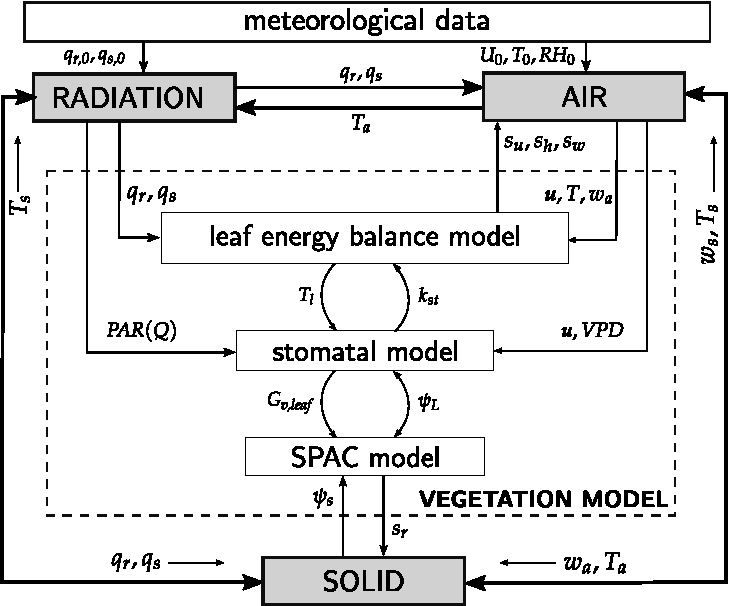
\includegraphics[width=\textwidth]{\figdir/fullmodelcoupling-crop.pdf}
	\caption{Coupling of the \textit{vegetation} model with \textit{air} domain solver, \textit{solid} domain solver, and the \textit{radiation} model. The parameters and the arrow indicate the transfer of information to couple the models. }
	\label{fig:fullmodelcoupling}
\end{figure}

The \textit{air} domain model describes the transport of moist air through vegetation (i.e., velocity, enthalpy, moisture content, and CO$_2$ concentration). Furthermore, with the air domain, the \textit{leaf energy balance} (LEB) model is solved to determine the heat and mass fluxes, which provides the necessary source and sink terms for solving the moist airflow. A summary of the leaf energy balance and the coupling between the air domain is provided in \cref{sec:airdomain}. The \textit{solid} domain model described the coupled heat and mass transport (i.e., solid temperature, and solid moisture content) in all urban materials (i.e., soil, pavement, and building facades). Furthermore, in the soil region which consists of vegetation roots, the \textit{soil-plant-atmosphere continuum} (SPAC) is solved to determine the leaf water potential (see \cref{sec:spac}) and the root water uptake, which provides the necessary sink term in soil region. A detailed description of the solid domain, SPAC model, and the coupling between them is provided in \cref{sec:soliddomain,sec:spac,sec:couplingalgorithm}, respectively. The final ingredient is the \textit{radiation} model which calculates the short-wave and long-wave radiative exchanges in the urban street canyon including the impact of vegetation. A detailed description of the radiation model is given in \cref{sec:radiationmodel}.

\section{Air domain: Transport of moist air}
\label{sec:airdomain}
The simplified vegetation model is described in \cref{ch:parametricstudy}, introduction the governing equation for moist flow through vegetation. The vegetation model, consisting of the ``\textit{leaf energy balance}'' (LEB) model, provides the necessary source (or sink) terms for heat, mass and momentum exchanges between vegetation and air as described in \cref{sec:cons_incompressible}. For the reader, a detailed derivation of the thermodynamics of the moist air is given in \cref{app:thermodynamics} and a detailed derivation of the governing equation of moist flow is given in \cref{app:conservation}. In this section, we summarize the pseudo-compressible form of governing equation for moist flow through vegetation where the buoyancy force is directly obtained from the density field.  


\subsection*{Conservation of species}
The governing equation consists of conservation of mass, momentum, energy, and species. The conservation equations are given in differential form in a Cartesian coordinate system described by the triplet $\mvec{x} = (x,y,z)$. In our study, the species of interest is water vapor (subscript $v$) and carbon-dioxide (CO$_2$) (subscript $c$). The conservation of species $i$ is given as:
\begin{equation}
\frac{\partial \rho x_i}{\partial t} + \nabla  \cdot \left( \rho x_i \mvec{u} \right) = - \nabla \cdot \mvec{g}_{\textit{d,i}} + s_i
\label{eq:xi}
\end{equation}
where $x_i$ is the concentration of species $i$, $\mvec{u} = \left(u,v,w\right)$ is the fluid velocity, $\mvec{g}_{\textit{d,i}}$ is the diffusive mass flux of the species, and $s_i$ is the source term. We assume that moist air is composed of dry air $a$, water vapor $v$ and carbon-dioxide $c$. The mass fraction of each component is:
\begin{align}
x_a &= \frac{\rho_a}{\rho} \\
x_v &= \frac{\rho_v}{\rho} \label{eq:xv}\\
x_c &= \frac{\rho_c}{\rho}\label{eq:xc}
\end{align}
and satisfies:
\begin{equation}
x_a + x_v + x_c = 1
\label{eq:massfrac}
\end{equation}
where $\rho_a$, $\rho_v$, $\rho_c$ are partial density of dry air, water vapor and CO$_2$ (kg\,m$^{-3}$). However, as $x_c \ll (x_a+x_v)$, we can approximate \cref{eq:massfrac} to:
\begin{equation}
x_a + x_v \approx 1
\end{equation}
Similarly, total density of gas mixture $\rho$ is given as:
\begin{equation}
\rho \approx \rho_a + \rho_v
\label{eq:rho2}
\end{equation} 

The Fick's law of diffusion is used to describe the diffusive mass flux as a function of concentration gradient of the species:
\begin{equation}
\mvec{g}_{\textit{d,i}} = - \rho D_{\textit{ia}} \nabla x_i
\label{eq:dmf}
\end{equation}
where $D_{ai}$ is the binary diffusion coefficient of species $i$ in air. Thus, substituting mass fractions \cref{eq:xv,eq:xc}, and diffusion mass flux \cref{eq:dmf} into \cref{eq:xi}, the conservation equation of species become:
\begin{align}
\frac{\partial \rho w}{\partial t} + \nabla  \cdot \left( \rho w \mvec{u} \right) &= D_{\textit{va}} \nabla^2 w + s_w \label{eq:xv2}\\
\frac{\partial \rho c}{\partial t} + \nabla  \cdot \left( \rho c \mvec{u} \right) &= D_{\textit{ca}} \nabla^2 c + s_c \label{eq:xc2}
\end{align}
where $s_w$ and $s_c$ are source of water and CO$_2$, respectively (see \cref{sec:leafenergy}). The notations $w\equiv x_v$ (kg\,kg$^{-1}$) and $c\equiv x_c\, M_a/M_c $ (mol\,mol$^{-1}$) are used to conform with past studies \citep{Carmeliet2005, Defraeye2011, Saneinejad2013, Kubilay2014b}.

\subsection*{Conservation of mass}

A detailed derivation of conservation of mass is given in \cref{sec:conservationofmass}. The conservation of mass for compressible moist flow is given as:
\begin{equation}
\frac{\partial \rho}{\partial t} + \nabla \cdot \left( \rho \mvec{u} \right) = 0
\end{equation}
where $\rho$ is defined by \cref{eq:rho2} and as $\mathcal{O}(s_w)\approx \num{e-4}$ (\cref{app:conservation}). We assume source of water vapor and CO$_2$ is negligible in conservation of mass. 

\subsection*{Conservation of momentum}

A detailed derivation of conservation of momentum is given in \cref{sec:conservationofmomentum}. The conservation of momentum is given as:
\begin{equation}
\frac{\partial \rho \mvec{u}}{\partial t} + \nabla  \cdot \left( \rho \mvec{u} \mvec{u} \right) = -\nabla p + \mu \nabla^2 \mvec{u} + \rho \mvec{g} + \mvec{s}_u
\end{equation}
where $p$ is the pressure (Pa), $\mu$ the dynamic viscosity (kg\,m$^{-1}$\,s$^{-1}$), $\mvec{g}$ the gravitational acceleration (m\,s$^{-2}$). The source of momentum $\mvec{s}_u$ is:
\begin{equation}
\mvec{s}_u = - \rho\, a \,c_d \,|\mvec{u}|\mvec{u}
\label{eq:suu}
\end{equation}
where $a$ is the leaf area density (m$^2$\,m$^{-3}$), and $c_d$ is the leaf drag coefficient ($c_d = 0.2$) \citep{Wilson1977} and is typically assumed to be a constant. It is done so in the present study for simplicity, but future studies can investigate the influence of varying drag coefficient. For turbulent flows, the viscous drag can be assumed to be negligible compared to the form drag \citep{Judd1996, Li1990, Liu1996}. 

\subsection*{Conservation of energy}

A detailed derivation of conservation of energy is given in \cref{sec:conservationofenergy}. The conservation of energy is given as:
\begin{equation}
c_p  \left( \frac{\partial }{\partial t} \left( \rho T \right) + \nabla \cdot \left(\rho T \mvec{u} \right)  \right) = - \nabla  \cdot \left(\lambda \nabla T \right) + \underbrace{a\,q_{\textit{sen,leaf}}}_{s_h}
\end{equation}
where $\rho$ (kg\,m$^{-3}$) is the density of mixture and $c_p$ (J\,kg$^{-1}$\,K$^{-1}$) is the specific heat capacity of the mixture. The source of energy $s_h$ (W\,m$^{-3}$) for the above equation (i.e., quasi- transport of temperature) is:
\begin{equation}
\mvec{s}_h = a\, q_{\textit{sen,leaf}}
\label{eq:sh}
\end{equation}
assuming that the sensible heat flux is only due to leaf and air thermal conduction (see \cref{sec:conservationofenergy} for detailed derivation). 

The (specific) enthalpies of dry air $h_a$ (J,kg$^{-1}$) and water vapor $h_v$ (J,kg$^{-1}$) are:
\begin{align}
h_a &= c_{pa} \left(T - T_{\mathit{ref}}\right) \\
h_v &= c_{pv} \left(T - T_{\mathit{ref}}\right) + L_v
\end{align}
where $L_v$ is the latent heat of vaporization. Thus, the total enthalpy of moist air is:
\begin{equation}
h \equiv \sum_i h_i x_i = c_p \left(T - T_{\mathit{ref}}\right) + L_v x_v
\end{equation}
where $c_p = x_a c_{\textit{pa}} +  x_v c_{\textit{pv}}$ is the specific heat capacity of gas mixture.

\subsection*{Turbulence modeling}

The Reynolds decomposition splits the instantaneous velocity into mean and fluctuating component:
\begin{equation}
\mvec{u} \left(\mvec{x},t\right) = \overline{\mvec{u}} \left(\mvec{x}\right) + \mvec{u}' \left(\mvec{x},t\right).
\end{equation}

Applying this averaging operator to the NS equations, resulting Reynolds-Averaged Navier-Stokes (RANS) equation is given as:
\begin{equation}
\frac{\partial \overline{\rho}}{\partial t} + \nabla \cdot \left(\overline{\rho}\,\overline{\mvec{u}}\right) = 0,
\end{equation}
\begin{equation}
\frac{\partial \overline{\rho}\,\overline{\mvec{u}}}{\partial t}  + \nabla \cdot \left(\overline{\rho}\,\overline{\mvec{u}}\,\overline{\mvec{u}}\right) = -\nabla \overline{p} + \mu \nabla^2 \overline{\mvec{u}} - \nabla \cdot \left(\overline{\rho \mvec{u}' \mvec{u}'}\right)+ \rho \mvec{g} + s_u
\end{equation}
where $\overline{\rho \mvec{u}' \mvec{u}'}$ is the Reynolds stresses. The Reynolds stresses are modeled using Bousinessq eddy-viscosity assumption:
\begin{equation}
- \overline{\rho \mvec{u}' \mvec{u}'} = \mu_t \left(\nabla u + \nabla u^T\right) - \frac{2}{3}\rho k \mvec{I}
\end{equation}
where:
\begin{equation}
\mu_t = \rho C_\mu \frac{k^2}{\varepsilon}
\end{equation}

In this study, we employ realizable $k-\varepsilon$ equations for determining the eddy-viscosity. The system of equations is given as:
\begin{align}
\frac{{\partial \rho k}}{{\partial t}} + \nabla \cdot \left(\rho k \tavg{\mvec{u}} \right)   &= \nabla  \cdot \left[ {\left( {\mu  + \frac{{{\mu _t}}}{{{\sigma _k}}}} \right)\nabla k} \right] + {P_k} - \rho \varepsilon  + s_k,\\
\frac{{\partial \rho \varepsilon }}{{\partial t}} +  \nabla \cdot \left(\rho \varepsilon \tavg{\mvec{u}} \right) &= \nabla  \cdot \left[ {\left( {\mu  + \frac{{{\mu _t}}}{{{\sigma _\varepsilon }}}} \right)\nabla \varepsilon } \right] + \rho{C_{1\varepsilon }}{P_k}\frac{\varepsilon }{k} - \rho{C_{2\varepsilon }}\frac{{{\varepsilon ^2}}}{{k + \sqrt {\nu \varepsilon } }} + s_\varepsilon
\label{eq:realizablekepsilon2}
\end{align}
where 
\begin{equation}
P_k = - \rho \overline{\mvec{u}'\mvec{u}'}:\nabla \tavg{\mvec{u}} = 2 \mu_t |\mathbf{S}|^2
\end{equation}
The mean strain-rate $\mathbf{S}$ is defined as
\begin{equation}
\mathbf{S} = \frac{1}{2} \left( \nabla \tavg{\mvec{u}} +  \nabla \tavg{\mvec{u}}^T \right)
\end{equation}

The TKE source $s_k$ (W\,m$^{-3}$) is given as: 
\begin{equation}
s_k = \rho {c_d}a\left( \beta _p \left| \tavg{\mvec{u}} \right|^3 - \beta _d\left| \tavg{\mvec{u}} \right|k \right)
\label{eq:source_k}		 	
\end{equation}
and the TDR source term $s_{\varepsilon}$ (W\,m$^{-3}$\,s$^{-1}$) is given as:
\begin{equation}
s_\varepsilon = \rho {c_d}a\left( {{\beta _p}{C_{4\varepsilon }}{{\left| \tavg{\mvec{u}} \right|}^3}\frac{\varepsilon }{k} - {\beta _d}{C_{5\varepsilon }}\left| \tavg{\mvec{u}} \right|\varepsilon } \right)
\label{eq:source_eps}		 	
\end{equation}
with model constants $C_{4\varepsilon}=0.9$ and $C_{5\varepsilon}=0.9$ \citep{Katul2004, Kenjeres2013, Sanz2003}. The constant $\beta_p=1.0$ is the fraction of mean kinetic energy converted into turbulent kinetic energy and $\beta_d=5.1$ describes the reduction in TKE and TDR due to vegetation \citep{Sanz2003}. \cite{Kenjeres2013} compared various RANS model coefficients for vegetation in an urban area and found the coefficients provided by \cite{Katul2004} to be reasonably accurate showing good numerical stability. Therefore, these parameters are used in this thesis.

\section{Leaf energy balance}
\label{sec:leafenergy}

The heat and mass exchanges between the tree canopy and the air are simulated using a leaf energy model. The heat and mass exchanges between the tree canopy and the air are simulated using a leaf energy balance as shown in \cref{fig:leaf_energybalance}. We assume a stationary leaf energy balance and that the dynamic thermal storage of heat in leaves can be neglected.

\begin{figure}[h]
	\centering
	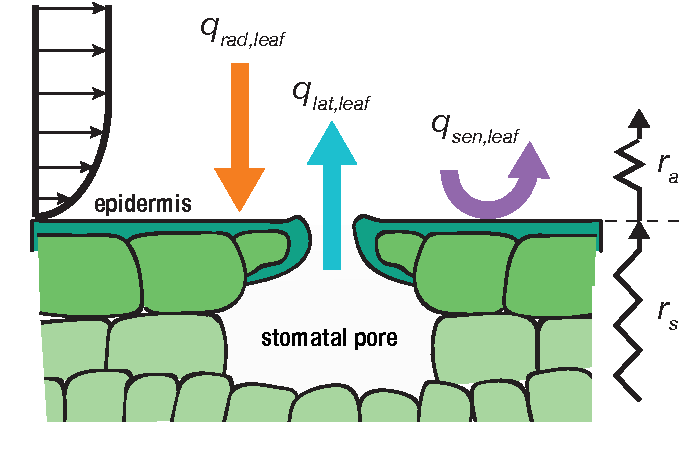
\includegraphics[width=0.8\textwidth]{\figdir/leafsurface-crop.pdf}
	\caption{Schematic representation of leaf surface with energy balance as given by \cref{eq:energybalance}. The radiative flux $q_{\mathit{rad,leaf}}$  absorbed by the leaf is balanced by the sensible $q_{\mathit{sen,leaf}}$ and the latent heat flux $q_{\mathit{lat,leaf}}$ leaving the leaf surface. The stomatal resistance 
		$r_s$ influences the latent heat flux and the aerodynamic resistance $r_a$ influences both the sensible and the latent heat fluxes. }
	\label{fig:leaf_energybalance}
\end{figure}

The stationary energy balance is given as:
\begin{equation}
{q_{\mathit{rad},\mathit{leaf}}} - {q_{\mathit{lat},\mathit{leaf}}} - {q_{\mathit{sen},\mathit{leaf}}} = 0
\label{eq:energybalance}
\end{equation}
where ${q_{\mathit{rad},\mathit{leaf}}}$ (W\,m$^{-2}$) is the radiative flux, ${q_{\mathit{sen},\mathit{leaf}}}$ (W\,m$^{-2}$) is the sensible heat flux and ${q_{\mathit{lat},\mathit{leaf}}}$ (W\,m$^{-2}$) is the latent heat flux \citep{Majdoubi2009, Bruse1998, Dauzat2001,Hiraoka2005}. Positive sensible and latent heat fluxes are defined as heat transfer from the leaf into the air. The sensible heat flux due to convective heat transfer from leaf surface to the air is given as:
\begin{equation}
{q_{\mathit{sen,leaf}}} = {h_{c,h}} \left( {{T_{\mathit{leaf}}} - T} \right) = \frac{{2\rho {c_p}}}{{{r_a}}} \left( {{T_{\mathit{leaf}}} - T} \right)
\label{eq:sensibleheatflux}
\end{equation}
where $h_{c,h}$ (W\,m$^{-2}$\,K$^{-1}$] is the convective heat transfer coefficient (CHTC), $T_{\mathit{leaf}}$ (K) is the leaf surface temperature, $T$ (K) is the air temperature and $r_a$ (s\,m$^{-1}$) is the aerodynamic resistance of the boundary layer around the leaf. A factor 2 is present in the equation as the sensible heat flux occurs on both sides of the leaf. Substituting \cref{eq:sensibleheatflux} into \cref{eq:sh} gives the source of heat from vegetation in conservation of energy.

The aerodynamic resistance $r_a$ (s\,m$^{-1}$) is given as \citep{Dauzat2001, Robitu2006}:
\begin{equation}
{r_a} = C\;{\left( {\frac{l}{{\left| {\bar{\mvec{u}}} \right|}}} \right)^{1/2}}
\label{eq:ra}
\end{equation}
where $C=130$ s$^{0.5}$\,m$^{-1}$ is the proportionality factor and $l$ (m) is the characteristic leaf size ranging from 0.02 m for conifers and up to 0.5 m for tropical plants \citep{Bruse1998}. The latent heat flux from leaf to air due to transpiration is defined as:
\begin{equation}
{q_{lat,leaf}} = {L_v} \, {g_{v,leaf}}
\label{eq:latentheatflux}
\end{equation}
where $L_v=\num{2.5e6}$ J kg$^{-1}$ is latent heat of vaporization. The water vapor flux $g_{v,leaf}$ (kg\,m$^{-2}$\,s$^{-1}$) is defined as:
\begin{equation}
{g_{\mathit{v,leaf}}} = {h_{c,m}}\left( {{p_{\mathit{v,leaf}}} - {p_v}} \right) = M_w\, k_{\textit{st,v}}^* \left( \frac{p_{\textit{v,i}} - {p_v}}{p} \right)
\label{eq:vapourflux2}
\end{equation}
where $h_{c,m}$ (s\,m$^{-1}$) is the convective mass transfer coefficient (CMTC), $M_w = \num{1.8015e-2}$ (kg\,mol$^{-1}$) is molar mass of water vapor, $p_{\textit{v,i}}$ (Pa) is the intercellular vapor pressure, $p_v$ (Pa) is the ambient vapor pressure, $p$ (Pa) is the ambient pressure, and $k_{\textit{st,v}}^*$ (mol\,m$^{-2}$\,s$^{-1}$) is the effective stomatal conductance of water vapor. A detailed description of the stomatal conductance is given in \cref{subsec:sm}. The energy balance (\cref{eq:energybalance}) is solved once the leaf surface temperature $T_{\mathit{leaf}}$ is known. Combining \cref{eq:energybalance,eq:sensibleheatflux,eq:latentheatflux}, the leaf temperature is given as:
\begin{equation}
{T_{\mathit{leaf}}} = T + \frac{{{q_{\mathit{rad,leaf}}} - {q_{\mathit{lat,leaf}}}}}{{{h_{c,h}}}}
\label{eq:solveleaft}
\end{equation}
where the equation is solved iteratively as $q_{\mathit{lat,leaf}}$ is dependent on the leaf temperature.

So, the source of moisture in the air domain, i.e., \cref{eq:xv2}, is obtained from \cref{eq:vapourflux2} as:
\begin{equation}
s_w = a\,{g_{\mathit{v,leaf}}}
\label{eq:sw}
\end{equation}
where $s_w$ (kg\,m$^{-3}$\,s${-1}$) is the moisture source term. In the present study, we assume that there is no condensation or rain on the leaf surface and so evapotranspiration is only due to transpiration through the leaf stomata. Therefore, the vapor pressure at the leaf is the vapour pressure within the leaf stomata which is close to the saturation vapor pressure at the leaf temperature, thereby we can assume
\begin{equation}
p_{\mathit{v,leaf}}\cong p_{\mathit{vsat,stom}} \left(T_{\mathit{leaf}}\right)
\end{equation}

%The water vapor mass flux $g_{\mathit{v,leaf}}$ (kg\,m$^{-2}$\,s$^{-1}$) from leaf into the air is given as:
%\begin{equation}
%{g_{\mathit{v,leaf}}} = {h_{c,m}}\left( {{p_{\mathit{v,leaf}}} - {p_v}} \right) = \frac{{\rho {R_a}}}{{p{R_v}}} \, \frac{1}{{{r_a} + {r_s}}}\left( {{p_{\mathit{v,leaf}}} - {p_v}} \right)
%\label{eq:vapourflux}
%\end{equation}
%where $h_{c,m}$ (s\,m$^{-1}$) is the convective mass transfer coefficient (CMTC), $p_{\mathit{v,leaf}}$ (Pa) is the vapor pressure at the leaf, $p_v$ (Pa) is the vapor pressure of the air above the leaf boundary layer, $r_s$ (s\,m$^{-1}$) is the stomatal resistance and $R_a=287.042$ J\,kg$^{-1}$\,K$^{-1}$ and $R_v=\num{461.524}$ J kg$^{-1}$~K$^{-1}$ are the gas constants of dry air and water vapor, respectively.

%The additional resistance $r_s$ is due to the stomatal regulatory control of the leaf. In the present study, the stomatal resistance is modeled as a function of climatic conditions: $q_{\mathit{r,sw}}$ the short-wave radiative flux in the air and $D$ (kPa) the vapor pressure deficit in the air, the difference between the saturation vapor pressure and the vapor pressure of the air
%\begin{equation}
%D \equiv p_{\mathit{v,sat}} - p_v
%\end{equation}


%\subsection*{Leaf energy balance}

%The \textit{leaf energy balance} (LEB) is summarized as:
%\begin{equation}
%{q_{\mathit{rad},\mathit{leaf}}} - {q_{\mathit{lat},\mathit{leaf}}} - {q_{\mathit{sen},\mathit{leaf}}} = 0
%\label{eq:energybalance2}
%\end{equation}
%where ${q_{\mathit{rad},\mathit{leaf}}}$ (W\,m$^{-2}$) is the radiative heat flux, ${q_{\mathit{lat},\mathit{leaf}}}$ (W\,m$^{-3}$) is the latent heat flux, and ${q_{\mathit{sen},\mathit{leaf}}}$ (W\,m$^{-3}$) is the sensible heat flux. The sensible heat flux is defined as:
%\begin{equation}
%{q_{\mathit{sen,leaf}}} = {h_{c,h}} \left( {{T_{\mathit{l}}} - T_a} \right)
%\label{eq:sensibleheatflux2}
%\end{equation}
%where $T_l$ (K) is the leaf temperature, $T_a$ (K) is the ambient temperature, and ${h_{c,h}}$ (W\,m$^{-2}$\,K$^{-1}$) is the convective heat transfer coefficient. Substituting \cref{eq:sensibleheatflux2} into \cref{eq:sh} gives the source of heat from vegetation in conservation of energy.

%The latent heat flux is defined as:
%\begin{equation}
%{q_{lat,leaf}} = {L_v} \, {g_{v,leaf}}
%\label{eq:latentheatflux2}
%\end{equation}
%where $L_v=\num{2.5e6}$ J\,kg${-1}$ is the latent heat of vaporization. The water vapor flux $g_{v,leaf}$ (kg\,m$^{-2}$\,s$^{-1}$) is defined as:
%\begin{equation}
%{g_{\mathit{v,leaf}}} = M_w\, k_{\textit{st,v}}^* \left( \frac{p_{\textit{v,i}} - {p_v}}{p} \right)
%\label{eq:vapourflux2}
%\end{equation}
%where $M_w = \num{1.8015e-2}$ (kg\,mol$^{-1}$) is molar mass of water vapor, $p_{\textit{v,i}}$ (Pa) is the intercellular vapor pressure, $p_v$ (Pa) is the ambient vapor pressure, and $k_{\textit{st,v}}^*$ (mol\,m$^{-2}$\,s$^{-1}$) is the effective stomatal conductance of water vapor. A detailed description of the stomatal conductance is given in \cref{subsec:sm}. So, the source of moisture in the air domain, i.e., \cref{eq:xv2}, is obtained from \cref{eq:vapourflux2} as:
%\begin{equation}
%s_w = a\,{g_{\mathit{v,leaf}}}
%\label{eq:sw}
%\end{equation}
%where $s_w$ (kg\,m$^{-3}$\,s${-1}$) is the moisture source term. 

Similarly, the CO$_2$ source in \cref{eq:xc2} is given as:
\begin{equation}
s_c = a\,{g_{\mathit{c,leaf}}} \frac{M_a}{M_c}
\end{equation}
where ${g_{\mathit{c,leaf}}}$ (kg\,m$^{-2}$\,s$^{-1}$) is the CO$_2$ flux from the leaf due to photosynthesis and also known as the assimilation rate (i.e., $A_n$). It is defined as:
\begin{equation}
{g_{\mathit{c,leaf}}} = M_c\, k_{st}^* \left( c_i - c \right)
\label{eq:co2flux}
\end{equation}
where $k_{st}^*$ (mol\,m$^{-2}$\,s$^{-1}$) is the effective stomatal conductance of CO$_2$, $c_i$ is intercellular CO$_2$ (mol\,mol$^{-1}$) concentration, and $c$ (mol\,mol$^{-1}$) is the ambient CO$_2$ concentration. A detailed description of assimilation rate is given in \cref{subsec:sm}.

\section{Solid domain: Coupled heat and moisture transport}
\label{sec:soliddomain}
\subsection{Composition of the porous material}

The building materials and the soil are considered as porous materials consisting of three phases: solid phase (denoted with $s$), liquid phase referring to liquid water ($l$) and the air phase which is split into dry air ($a$) and water vapor $v$ \citep{Defraeye2011, Saneinejad2013, Carmeliet2005,Janssen2002}. The open porosity $\phi_o$ (m$^3$\,m$^{-3}$) of the porous material is defined as:
\begin{equation}
\phi_o = \frac{V_{\mathit{pore}}}{V}
\end{equation}
where $V_{\textit{pore}}$ (m$^3$) is the volume of open pores and $V$ (m$^3$) is the total volume of the porous material $\tensor{S}$. The solid material content $w_s$ (kg\,m$^{-3}$) is defined as:
\begin{equation}
w_s = \left(1 - \phi_o \right) \rho_s
\end{equation}
where $\rho_s$ (kg\,m$^{-3}$) is the solid material matrix density. Similarly the dry air $w_a$, water vapor $w_v$, liquid water $w_l$ contents are defined as:
\begin{align}
w_l &= \phi_o S_l \rho_l \\
w_a &= \phi_o \left( 1 - S_l \right) \rho_a \\
w_v &= \phi_o \left( 1 - S_l \right) \rho_v
\end{align}
where they are related to the degree of liquid saturation $S_l$ of the porous open pores:
\begin{equation}
S_l = \frac{\phi_{\textit{o,l}}}{\phi_o}
\end{equation}
with $\phi_{\textit{o,l}}$ being the amount of liquid water occupied inside the open pores and $\rho_a$, $\rho_l$ being the air and liquid water densities, respectively. The total moisture content $w$ (kg\,m$^{-3}$) inside the porous material is simply the sum of liquid water and water vapor:
\begin{equation}
w = w_l + w_v
\end{equation}

\subsection{Water potential}

Water potential is a universal variable to determine the \textit{water status} in any medium \citep{nobel2009physicochemical}. In this thesis, we use it to define the water status of multiple domains such as solid porous materials (soil and building facades), plant xylem, and air. The water potential $\psi$ (Pa) describes the chemical potential of water $\mu$ (J\,mol$^{-1}$) with respect to chemical potential of pure water $\mu^{o,l}$ (J\,mol$^{-1}$) at the same temperature, standard atmosphere and at zero level:
\begin{equation}
\psi = \frac{\mu - \mu^{o,l}}{V^o_l}
\end{equation}
where $V^o_l = 18.05 \num{e-3}$ m$^3$\,mol$^{-1}$ is the molar volume of pure water in liquid phase. The water potential for pure water at standard atmosphere is $\psi = 0$ Pa. The water tends to move towards a region where $\mu-\mu^{o,l}$ is lower, i.e. in the direction of $-\nabla\psi$. The water potential is related to pressure potential, osmotic potential, matrix potential, and gravitational potential. In our study, we assume that the pressure potential gradient is negligible in the solid and we ignore the influence of osmotic potential $\psi_o$ (Pa) as we assume we have a non-saline porous material. Therefore, only the matrix potential and gravitation potential influence the water transport:
\begin{equation}
\psi = \underbrace{p_c}_{\psi_c} + \underbrace{\rho_l g z}_{\psi_g}
\end{equation}
where $\psi_c = p_c$ (Pa) is the capillary potential due to capillary pressure, which represents the contribution of the matrix potential, and $\psi_g = \rho_l g h$ (Pa) is the gravitational potential with $g = |\mvec{g}|$ (m\,s$^{-2}$) where $\mvec{g}$ is the gravitational acceleration. The capillary pressure $p_c$ is defined as the difference between liquid and gas phase pressure, $p_l$ and $p_g$, respectively:
\begin{equation}
p_c =  p_l - p_g
\end{equation}
and is related to relative humidity $\phi$ by the Kelvin's law:
\begin{equation}
p_c = \rho_l R_v T \ln \left(\phi\right)
\end{equation}

The gravitational potential $\psi_g$ (Pa) is defined as:
\begin{equation}
\psi_g = - \rho \mvec{g} \cdot \mvec{x} = \rho g z
\end{equation}
where $g = |\mvec{g}|$ with $z$ oriented upward. Thus, by taking the capillary and gravitational water potentials into account, the transport of water can be described in building materials and, more importantly, soil region where the plant roots are present.

\subsection{Coupled transport of heat and mass}
\label{subsec:ctoham}
\subsubsection*{Conservation of mass}
The conservation of mass in the solid domain is defined as:
\begin{align}
\pde{w_s}{t} &= 0 \label{eq:solidcom} \\ 
\pde{w_a}{t} + \nabla \cdot \left(w_a\mvec{u}_a \right) &= 0 \label{eq:aircom} \\ 
\pde{w_l + w_v}{t} + \nabla \cdot \left(w_l\mvec{u}_l + w_v\mvec{u}_v \right) &= 0 \label{eq:liqcom}
\end{align}
assuming that solid matrix does not change, mass of different phases only changes due to evaporation or condensation. Other phenomena such as melting, freezing, sublimation and deposition are neglected. Assuming dry air does not contribute to moisture storage, i.e., $\partial w_a / \partial t = 0$, the conservation of mass simplifies to rate of change of moisture content $w = w_l + w_v$, from \cref{eq:liqcom}:
\begin{equation}
 \pde{w}{t} = - \nabla \cdot \left(\mvec{g}_l + \mvec{g}_v \right)
\end{equation}
where $\mvec{g}_l \equiv w_l\mvec{u}_l$ (kg\,m$^{-2}$\,s$^{-1}$) and $\mvec{g}_v \equiv w_v\mvec{u}_v$ (kg\,m$^{-2}$\,s$^{-1}$) are defined as the liquid water and water vapor fluxes, respectively. Additionally, the plant transpiration leafs to root uptake leading to a water loss in the soil domain. The contribution of root water uptake due to plant transpiration is introduced through the source term $s_r$ (kg\,m$^{-3}$\,s$^{-1}$):
\begin{equation}
\pde{w}{t} = - \nabla \cdot \left(\mvec{g}_l + \mvec{g}_v \right) + s_r
\label{eq:com4}
\end{equation}

The sink term due to root water uptake is explained in detail later in \cref{sec:spac}. In this thesis, the conservation of mass is solved using the $p_c$-form Richards equation, where \cref{eq:com4} becomes:
\begin{equation}
\frac{\partial w}{\partial p_c} \frac{\partial p_c}{\partial t} = -  \nabla \cdot \left(\mvec{g}_l + \mvec{g}_v\right) + s_{r}
\label{eq:com5}
\end{equation}
with $C_{mm} \equiv \partial w/ \partial p_c$ (kg\,m$^{-3}$\,Pa$^{-1}$) is defined as the moisture capacity. Thus, the change in water content in the porous material is simply due to the liquid and vapor fluxes, and root water uptake (only in soil where root is present). The liquid water flux $\mvec{g}_l$ in porous media is given by:
\begin{equation}
\mvec{g}_l = - K_{\textit{lp}} \nabla \left(p_c + \rho_l g z\right)
\label{eq:liquidflux}
\end{equation}
and assumes the air pressure effects be negligible with respect to capillary and gravitational effects, where $K_{\textit{lp}}$ (s) is the liquid water permeability. We assume that the liquid water permeability is only due to pressure gradient, and the influence of thermal gradient is neglected \citep{Carmeliet2005}. The water vapor flux in the porous media is given by:
\begin{equation}
\mvec{g}_v = K_{\textit{vp}}\nabla p_c + K_{\textit{vT}}\nabla T
\label{eq:vaporflux}
\end{equation}
where
\begin{equation}
K_{\textit{vp}} = - \delta_v \frac{p_v}{\rho_l R_v T}
\end{equation}
is the water vapor permeability (s) due to pressure,  
\begin{equation}
K_{\textit{vT}} = - \delta_v \frac{p_v}{\rho_l R_v T^2}\left(\rho_l L_v - p_c\right)
\end{equation}
is the water vapor permeability (s) due to temperature gradient, and
\begin{equation}
\delta_v = \frac{D_{\textit{va,mat}}}{R_v T}
\end{equation}
is the water vapor diffusion coefficient (s) where $D_{\textit{va,mat}}$ (m$^2$\,s$^{-1}$) is the binary apparent diffusion coefficient between dry air and water vapor \citep{Carmeliet2005, Defraeye2011, Saneinejad2013, Kubilay2014b}. Thus, substituting the fluxes \cref{eq:liquidflux,eq:vaporflux} into \cref{eq:com5}, the expanded form of conservation of mass is given as:
\begin{equation}
C_{\textit{mm}}\frac{\partial p_c}{\partial t} = \nabla \cdot \Big( K_{lp} \nabla \left(p_c + \rho_l g z\right) + K_{\textit{vp}}\nabla p_c + K_{\textit{vT}}\nabla T \Big) + s_r
\label{eq:com6}
\end{equation}

\subsubsection*{Conservation of energy}
The conservation of energy is given as:
\begin{equation}
\frac{\partial h}{\partial t} + \nabla \cdot \left(h \mvec{u}\right) = - \nabla \cdot \mvec{q}
\label{eq:coe1}
\end{equation}
where $h$ (J\,kg$^{-1}$) is the enthalpy of total solid domain:
\begin{equation}
h = \sum_i w_i h_i = w_s h_s + w_a h_a + w_l h_l + w_v h_v
\label{eq:enthalphy1}
\end{equation}
and heat conduction $\mvec{q}$ (W\,m$^{-2}$) is given by Fourier's law as:
\begin{equation}
\mvec{q} = -\lambda \nabla T
\label{eq:fourierlaw}
\end{equation}
where $T$ (K) is temperature, $\lambda$ (W\,m$^{-1}$\,K$^{-1}$) is thermal conductivity.

Substituting \cref{eq:enthalphy1} into \cref{eq:coe1} expands to:
\begin{equation}
\frac{\partial}{\partial t}\left(w_s h_s + w_a h_a + w_l h_l + w_v h_v \right) + \nabla \cdot \left(w_a \mvec{g}_a + w_l \mvec{g}_l + w_v \mvec{g}_v\right) = - \nabla \cdot \mvec{q}
\label{eq:coe1p1}
\end{equation}
and assuming dry air and water vapor does not contribute to heat storage, i.e., $\partial w_a h_a / \partial t \approx 0$ and $\partial w_v h_v / \partial t \approx 0$, and convection term of dry air is negligible $\nabla \cdot w_a \mvec{g}_a \approx 0$, \cref{eq:coe1p1} simplified to:
\begin{equation}
\frac{\partial \left(w_s h_s + w_l h_l \right)}{\partial t} + \nabla \cdot \left(w_l \mvec{g}_l + w_v \mvec{g}_v\right) = - \nabla \cdot \mvec{q}
\label{eq:coe1p2}
\end{equation}

The enthalpies of solid $h_s$, liquid water $h_l$ and water vapor $h_v$ are defined as:
\begin{align}
h_s &= c_{ps} \left(T - T_{\textit{ref}}\right) \label{eq:enthalphys}\\
h_l &= c_{pl} \left(T - T_{\textit{ref}}\right) \label{eq:enthalphyl}\\
h_v &= c_{pv} \left(T - T_{\textit{ref}}\right) + L_v \label{eq:enthalphyv}
\end{align}
and $L_v$ is the latent heat of vaporization of water. Substituting \cref{eq:enthalphys,eq:enthalphyl,eq:enthalphyv} into \cref{eq:coe1p2}, the conservation of energy is given as:
\begin{equation}
\begin{split}
&\left(c_{\textit{ps}} w_s + c_{\textit{pl}} w\right)\frac{\partial T}{\partial t} + \left[c_{pl} \left(T - T_{\textit{ref}}\right) \frac{\partial w}{p_c}\right]\frac{\partial p_c}{\partial t} =\\
& - \nabla \cdot \bigg\{ {\mvec{q} + \underbrace{ c_{\textit{pl}} \left(T - T_{\textit{ref}}\right)\mvec{g}_l}_{\mvec{q}_l} + \underbrace{ \Big[c_{\textit{pv}} \left(T - T_{\textit{ref}}\right) + L_v\Big]\mvec{g}_v}_{\mvec{q}_v} } \bigg\}
\end{split}
\label{eq:coe3}
\end{equation}

We defined the thermal capacity terms as:
\begin{align}
C_{\textit{TT}} &=  c_{\textit{ps}}w_s + c_{\textit{pl}}w \label{eq:cap1} \\
C_{\textit{Tp}} &=  c_{\textit{pl}} \left( T - T_{\mathit{ref}}\right) \pde{w}{p_c} \label{eq:cap2} 
\end{align}
are the thermal capacity terms. Substituting liquid and vapour fluxes, \cref{eq:liquidflux,eq:vaporflux}, respectively, thermal capacities \cref{eq:cap1,eq:cap2} and heat conduction \cref{eq:fourierlaw} into conservation of energy equation \cref{eq:coe3} we get:
\begin{align}
\begin{aligned}
		\mathllap{C_{\textit{TT}}\frac{\partial T}{\partial t} + C_{\textit{Tp}}\frac{\partial p_c}{\partial t}} = \nabla \cdot \bigg(\lambda \nabla T &+  K_{\textit{lp}} c_{\textit{pl}} \left(T - T_{\textit{ref}}\right) \left(\nabla p_c + \rho_l g z\right) \\
%					&+ K_{\textit{lp}} c_{\textit{pl}} \left(T - T_{\textit{ref}}\right) \\
					&- K_{\textit{vp}} \Big[c_{\textit{pv}} \left(T - T_{\textit{ref}}\right) + L_v\Big] \nabla p_c \\ 
					&- K_{\textit{vT}} \Big[c_{\textit{pv}} \left(T - T_{\textit{ref}}\right) + L_v\Big] \nabla T \bigg)
\end{aligned}
\end{align}
where the terms on RHS are heat transport due to conduction, liquid transport, and vapor transport.

\subsection{Linearized heat and mass transport equation}

In the present study, the conservation of mass and energy is coupled together as a heat and mass model (HAM) according to \citep{Janssen2002,Defraeye2011,Carmeliet2005,Saneinejad2013,Kubilay2018}. Due to the shape of the water retention curve and the hydraulic conductivity curve, as shown in \cref{fig:wrc}, the Richards equation is highly non-linear. Therefore, the numerical solution of the equation is very sensitive to convergence tolerance and requires linearization techniques to maintain accuracy and computational efficiency. Methods such as fixed-point Picard iterations are used to solve the non-linear equations. More details on the discretization is provided in \cite{Liu2012,Janssen2002,Kubilay2018}. 

The conservation of mass (i.e., the moisture transport equation), \cref{eq:com6}, in the linearized form is given as:
\begin{equation}
\begin{split}
C^{n+1,k}_{\textit{mm}}\frac{p_c^{n+1,k+1}-p_c^{n}}{\Delta t} = \nabla \cdot \Big( K_{\textit{lp}}^{n+1,k} &\nabla \left(p_c^{n+1,k+1} + \rho_l g z\right)\\
&+ K_{\textit{vp}}^{n+1,k} \nabla p_c^{n+1,k+1} \\
&+ K_{vT}^{n+1,k} \nabla T^{n+1,k}\Big)\\
+ s_r^{n+1,k+1}&
\end{split}
\end{equation}
where the capacity, permeabilities and temperature are determined from the previous Picard iteration ($k$). The subscript ($n$) denotes the global (i.e., outer) time step of $t$ and $k$ denoting the internal Picard iteration step. When the Picard solution approaches convergence, i.e., $p_c^{n+1,k} \rightarrow p_c^{n+1,k+1}$, $\partial{w}/\partial p_c$ becomes negligible resulting in larger mass conservation errors. The error is minimized by formulating the Richard's equation in mixed-form \citep{Liu2012}:
\begin{equation}
\begin{split}
C^{n+1,k}_{\textit{mm}}\frac{p_c^{n+1,k+1}-p_c^{n}}{\Delta t} = \nabla \cdot \Big( K_{\textit{lp}}^{n+1,k} &\nabla \left(p_c^{n+1,k+1} + \rho_l g z\right)\\
&+ K_{\textit{vp}}^{n+1,k} \nabla p_c^{n+1,k+1} \\
&+ K_{vT}^{n+1,k} \nabla T^{n+1,k}\Big)\\
+ s_r^{n+1,k+1} &- \frac{w^{n+1,k+1}-w^n}{\Delta t}
\end{split}
\end{equation}
where an additional moisture change term is added.

\begin{figure}[t]
	\centering
	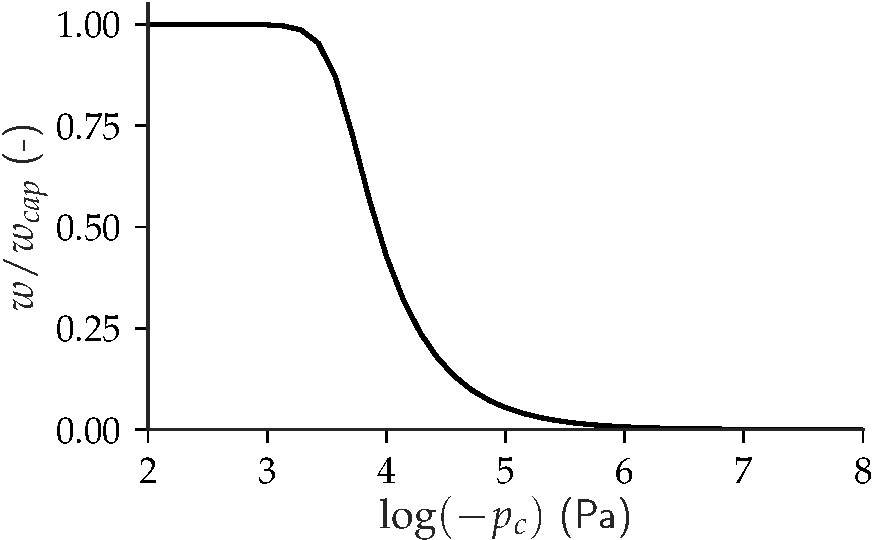
\includegraphics[width=0.5\textwidth]{\figdir/waterretentioncurve-crop.pdf}
	\caption{Typical non-linear moisture water retention curve for a material which is capillary saturated.}
	\label{fig:wrc}
\end{figure}

The linearized form of the heat equation is given as:
\begin{equation}
\begin{split}
	C_{\textit{TT}}^{n+1,k}& \frac{T^{n+1,k+1}-T^{n}}{\Delta t} = \nabla \cdot \bigg(\lambda \nabla T^{n+1,k+1} \\
	&+ K_{\textit{lp}}^{n+1,k} c_{\textit{pl}} \left(T^{n+1,k+1} - T_{\textit{ref}}\right)  \nabla p_c^{n+1,k+1} \\
	&+ K_{\textit{lp}}^{n+1,k} c_{\textit{pl}} \left(T^{n+1,k+1} - T_{\textit{ref}}\right) \rho_l g z\\
	&- K_{\textit{vp}}^{n+1,k} \Big[c_{\textit{pv}} \left(T^{n+1,k+1} - T_{\textit{ref}}\right) + L_v\Big] \nabla p_c^{n+1,k} \\ 
	&- K_{\textit{vT}}^{n+1,k} \Big[c_{\textit{pv}} \left(T^{n+1,k+1} - T_{\textit{ref}}\right) + L_v\Big] \nabla T^{n+1,k+1} \bigg)
\end{split}
\end{equation}
where the capillary pressure time derivative term is ignored. The mixed-form the heat equation is given as:
\begin{equation}
\begin{split}
C_{\textit{TT}}^{n+1,k}&\frac{T^{n+1,k+1}-T^{n}}{\Delta t} = \nabla \cdot \bigg(\lambda \nabla T^{n+1,k+1} \\
&+ K_{\textit{lp}}^{n+1,k} c_{\textit{pl}} \left(T^{n+1,k+1} - T_{\textit{ref}}\right)  \nabla p_c^{n+1,k+1} \\
&+ K_{\textit{lp}}^{n+1,k} c_{\textit{pl}} \left(T^{n+1,k+1} - T_{\textit{ref}}\right) \rho_l g z\\
&- K_{\textit{vp}}^{n+1,k} \Big[c_{\textit{pv}} \left(T^{n+1,k+1} - T_{\textit{ref}}\right) + L_v\Big] \nabla p_c^{n+1,k} \\
&- K_{\textit{vT}}^{n+1,k} \Big[c_{\textit{pv}} \left(T^{n+1,k+1} - T_{\textit{ref}}\right) + L_v\Big] \nabla T^{n+1,k+1} \bigg)\\
&- \frac{C_{TT}^{n+1}T^{n+1} - C_{TT}^{n}T^{n}}{\Delta t}
\end{split}
\end{equation}


The system of linear equations is solved by Krylov subspace iteration solver, i.e. preconditioned conjugate gradient (PCG) with diagonal-based incomplete Cholesky (DIG) preconditioning. The convergence criteria for the Picard iteration is user-defined: 
\begin{equation}
\left| p_c^{n+1,k+1} - p_c^{n+1,k}\right| \le \delta p_c
\end{equation}
\begin{equation}
\left| T^{n+1,k+1} - T^{n+1,k}\right| \le \delta T
\end{equation}
where $\delta p_c = \delta T = 10^{-2}$ \citep{Kubilay2018}.

\section{Soil-Plant-Atmosphere Continuum model}
\label{sec:spac}

The soil-plant-atmosphere continuum (SPAC) model that is integrated into the vegetation model is described in this section, implemented according to the state-of-art techniques: \citep{Volpe2013,Manoli2014,Launiainen2015,Idso1977,Manzoni2011,Farquhar1980}. The root-system of the plants are represented as a network-like structure assuming cooperative strategy among the individual roots and a bulk plant transpiration through the xylem system. We assume no water storage inside the plant and therefore, the water flux from soil to root $G_{\textit{v,root}}$, from root to leaf through xylem $G_{\textit{v,xylem}}$, and from leaf to air $G_{\textit{v,leaf}}$ is equal, as depicted in \cref{fig:SPAC_waterbalance}:
\begin{equation}
G_{\textit{v,root}} = G_{\textit{v,xylem}} = G_{\textit{v,leaf}}
\label{eq:massfluxeq}
\end{equation}
and so, the atmospheric evaporative demand (AED) is dependent on the water availability near the roots of the plants.

\begin{figure}[t]
	\centering
	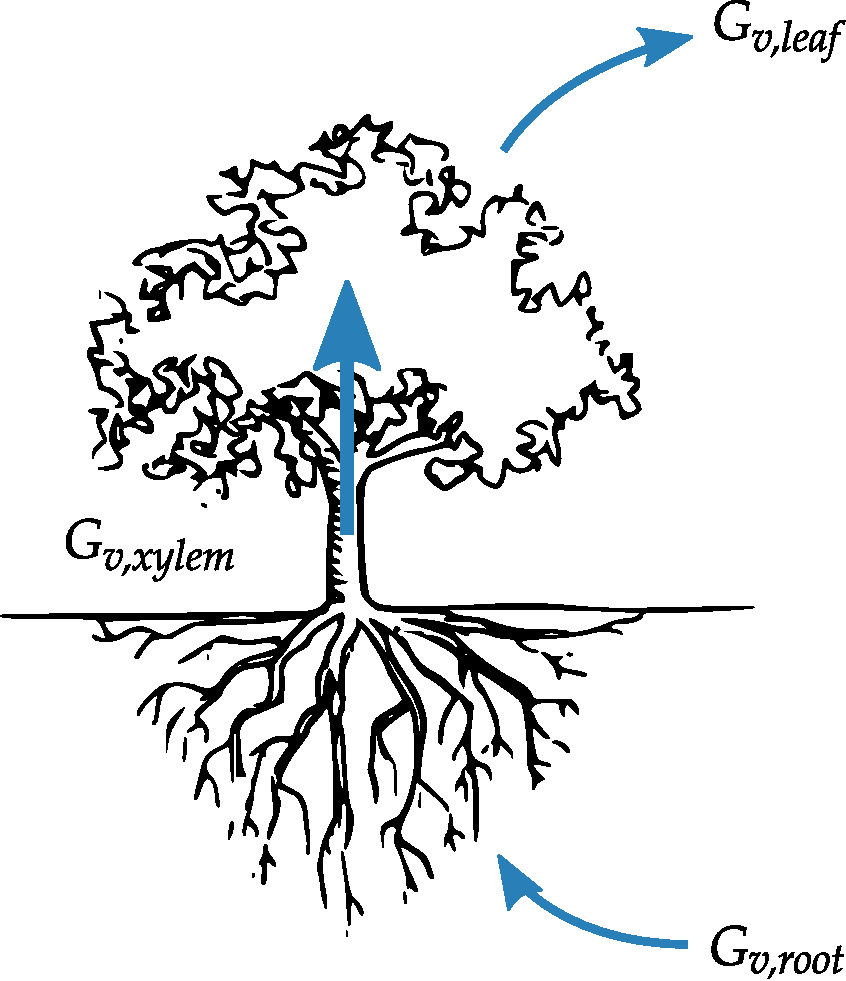
\includegraphics[width=0.5\textwidth]{\figdir/SPAC_waterbalance_v2-crop.pdf}
	\caption{Soil-Plant-Atmosphere Continuum: The water balance between plant transpiration and root water uptake, $G_{\textit{v,root}} = G_{\textit{v,xylem}} = G_{\textit{v,leaf}}$.}
	\label{fig:SPAC_waterbalance}
\end{figure}

\subsection{Water transport in soil-root system}

The sink term $s_r$ (kg\,m$^{-3}$\,s$^{-1}$) due to root water uptake in soil moisture transport equation (\cref{eq:com6}) is simply defined as:
\begin{equation}
s_r = r \, g_{\textit{v,root}}
\end{equation}
where $r$ (m$^2$\,m$^{-3}$) is the root area density and $g_{\textit{v,root}}$ (kg\,m$^{-2}$\,s$^{-1}$) is the root water uptake, i.e., the flux of water from root to soil. It is defined as:
\begin{equation}
g_{\textit{v,root}} = k_{sr}^*\left(\psi_s - \psi_R\right)
\end{equation}
where $k_{sr}^*$ (s\,m$^{-1}$) is effective conductance of the soil-root system (i.e., rhizosphere), $\psi_s$ (Pa) is the soil water potential, and $\psi_R$ (Pa) is the (bulk) root water potential. The effective conductance of the soil-root system (or rhizosphere) $k_{sr}^*$ (s\,m$^{-1}$) is given as:
\begin{equation}
k_{sr}^* = \frac{1}{|\mvec{g}|} \frac{k_s\,k_r}{k_s + k_r}
\end{equation}
where $\mvec{g}$ (m\,s$^{-2}$) is the gravitational acceleration, $k_s$ (s$^{-1}$) is the soil conductance in the root region, and $k_r$ (s$^{-1}$) is the conductance of the root system. The soil conductance in the root region $k_s$ (s$^{-1}$) is defined as:
\begin{equation}
k_s = \alpha \, K \, r
\end{equation}
where
\begin{equation}
\alpha =  \sqrt{\left(\frac{L}{\textit{RAI}}\right) \frac{1}{d}}
\end{equation}
$d$ (m) is the root diameter, $L$ (m) is the root-depth height, and $\textit{RAI} = \int r\,\mathrm{d}z$ is the root area index (m$^2$\,m$^{-2}$). The hydraulic conductivity in soil $K$ (m\,s$^{-1}$) is given as:
\begin{equation}
K = K_{\textit{lp}} \, |\mvec{g}|
\end{equation}
where $K_{\textit{lp}}$ (s) being the liquid permeability defined in the \cref{subsec:ctoham}. Finally, the conductance of the root system $k_r$ (s$^{-1}$) is given as:
\begin{equation}
k_r = r \frac{\Delta z}{\beta}
\end{equation}
where $\Delta z$ is the vertical height of the root layer mesh and $\beta = \num{3e8}$ s. 

\begin{figure}[t]
	\centering
	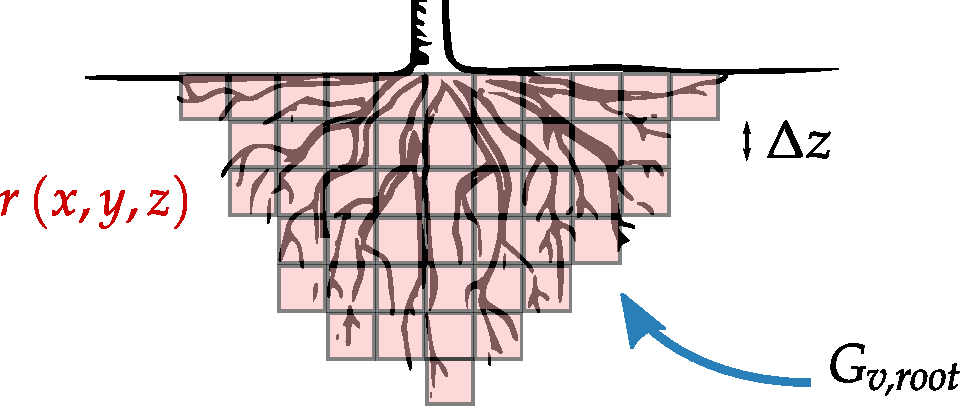
\includegraphics[width=0.65\textwidth]{\figdir/SPAC_root_v3-crop.pdf}
	\caption{Soil-Plant-Atmosphere Continuum: The water transport in soil-root system.}
	\label{fig:SPAC_root}
\end{figure}

Thus, the net root water uptake from the soil domain $G_{\textit{v,root}}$ (kg\,s$^{-1}$) is given as:
\begin{equation}
G_{\textit{v,root}} = \int_{\Omega_s} s_r\,\mathrm{d}V = \int_{\Omega_s} r\,g_{\textit{v,root}}\,\mathrm{d}V
\end{equation}
where $\Omega_s$ denotes the soil domain (note that as $r=0$ outside root-zone, the integration is essentially only in the root volume). 

%The water uptake from the root is equal to the water transport in the xylem as so:
%\begin{equation}
%G_{\textit{v,root}} = G_{\textit{v,xylem}}
%\end{equation}

\subsection{Water transport in xylem}

The water flux through the plant in xylem  layer $g_{\textit{v,xylem}}$ (kg\,m$^{-2}$\,s$^{-1}$) is defined as:
\begin{equation}
g_{\textit{v,xylem}}(\psi_L) = k_x^* \left(\psi_R - \psi_L\right)
\end{equation}
where $k_x^*$ (s\,m$^{-1}$) is the effective xylem conductance, $\psi_R$ (Pa) is the (bulk) root water potential, and $\psi_L$ (Pa) is the (bulk) leaf water potential. The net water flux $G_{\textit{v,xylem}}$ (kg\,s$^{-1}$) is given as:
\begin{equation}   
G_{\textit{v,xylem}} = \int_{\partial\Omega_{x|s}} g_{\textit{v,xylem}}~\mathrm{d}A = g_{\textit{v,xylem}} A_x
\label{eq:netwaterflux_xylem}
\end{equation}
where $A_x$ (m$^2$) is the xylem cross-sectional area. The effective xylem conductance $k_x^*$ (s\,m$^{-1}$) of water is:
\begin{equation}
k_x^* = k_x \, \rho_l
\end{equation}
where plant xylem conductance $k_x$ (m\,Pa$^{-1}$\,s$^{-1}$) is modeled using a ``\textit{vulnerability curve}'' approach. The xylem conductance becomes exponentially smaller with increasing leaf water potential \citep{Volpe2013}. This empirical model is based on plant response of the vulnerability to xylem cavitation and embolism that could occur at very low water potential. The xylem conductance $k_x$ (m\,Pa$^{-1}$\,s$^{-1}$) is defined by:
\begin{equation}
k_x = k_{\textit{x,max}} \exp \left\{ - \left( - \frac{\psi_L}{d}\right)^c \right\}
\end{equation}
where $k_{\textit{x,max}}$ (m\,Pa$^{-1}$\,s$^{-1}$) is the maximum xylem conductance, and $c$ and $d$ are fit-coefficients \citep{Volpe2013}.


\begin{figure}[t]
	\centering
	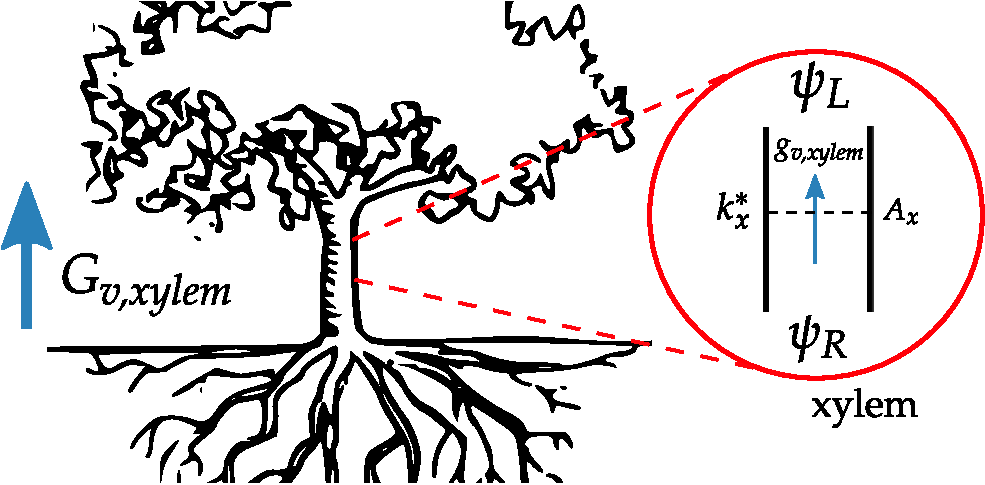
\includegraphics[width=0.65\textwidth]{\figdir/SPAC_xylem-crop.pdf}
	\caption{Soil-Plant-Atmosphere Continuum: The water transport in plant xylem.}
	\label{fig:SPAC_xylem}
\end{figure}

%Similarly, the net flux of water in xylem should be equal to the net transpiration rate, as storage is negligible. Therefore, 
%\begin{equation}
%G_{\textit{v,xylem}} = G_{\textit{v,leaf}}
%\end{equation}
%and moreover,
%\begin{equation}
%G_{\textit{v,root}}  = G_{\textit{v,xylem}} = G_{\textit{v,leaf}}
%\end{equation}

\subsection{Water transport from leaf to air}

The leaf transpiration rate $g_{\textit{v,leaf}}$ (kg\,m$^{-2}$s$^{-1}$) as defined in \cref{sec:airdomain}, \cref{eq:vapourflux2}, and is simply defined as:
\begin{equation}
g_{\textit{v,leaf}} = M_w\, k_{st,v}^* \left(\frac{p_{\textit{v,leaf}} - p_v}{p}\right)
\label{eq:gvleaf}
\end{equation}
where $p_{\textit{v,leaf}}$ (Pa) is the vapor pressure at the leaf, $p_v$ (Pa) is the ambient vapor pressure and $p$ (Pa) is ambient pressure. In plant-science community, the leaf transpiration is typically given in molar units ($f_c$ (mol\,m$^{-2}$\,s$^{-1}$)) and is obtained from \cref{eq:gvleaf}:
\begin{equation}
f_v = g_{\textit{v,leaf}} / M_w = k_{st,v}^* \left(\frac{p_{\textit{v,leaf}} - p_v}{p}\right)
\label{eq:fvorig}
\end{equation}

The effective stomatal conductance of water vapor $k_{st,v}^*$ (mol\,m$^{-2}$\,s$^{-1}$) is defined as:
\begin{equation}
k_{\textit{st,v}}^* = a_c \,k_{\textit{st}}^*
\end{equation}
where $k_{\textit{st}}^*$ (mol\,m$^{-2}$\,s$^{-1}$) is the effective stomatal conductance of CO$_2$, and $a_c = 1.6$ is the relative diffusion of water vapor to CO$_2$. The effective stomatal conductance is the sum of stomatal and boundary layer conductance (assumed to be in series):
\begin{equation}
k_{\textit{st}}^* = \frac{k_{\textit{st}}\,k_b}{k_{\textit{st}} + k_b}
\label{eq:ksteff}
\end{equation}
where $k_b$ (mol\,m$^{-2}$\,s$^{-1}$) is the boundary layer conductance (i.e. $g_b$ (in plant-science), or inverse of boundary layer resistance $r_b$, assumed to be equivalent to aerodynamic resistance $r_a$). \cref{eq:ksteff} given in terms of resistances is given as:
\begin{equation}
k_{\textit{st}}^* = \frac{1}{r_s + r_a}
\label{eq:hcm2}
\end{equation}
where $r_s$ (s\,m$^{-1}$)is the stomatal resistance.

%A factor 2 is present in the equation as the sensible heat flux occurs on both sides of the leaf. The aerodynamic resistance $r_a$ (s\,m$^{-1}$) is given as \citep{Dauzat2001, Robitu2006}:
%\begin{equation}
%{r_a} = C\;{\left( {\frac{l}{{\left| {\bar{\mvec{u}}} \right|}}} \right)^{1/2}}
%\label{eq:ra2}
%\end{equation}
%where $C=130$ s$^{0.5}$\,m$^{-1}$ is the proportionality factor and $l$ (m) is the characteristic leaf size ranging from 0.02 m for conifers and up to 0.5 m for tropical plants \citep{Bruse1998}.


\begin{figure}[t]
	\centering
	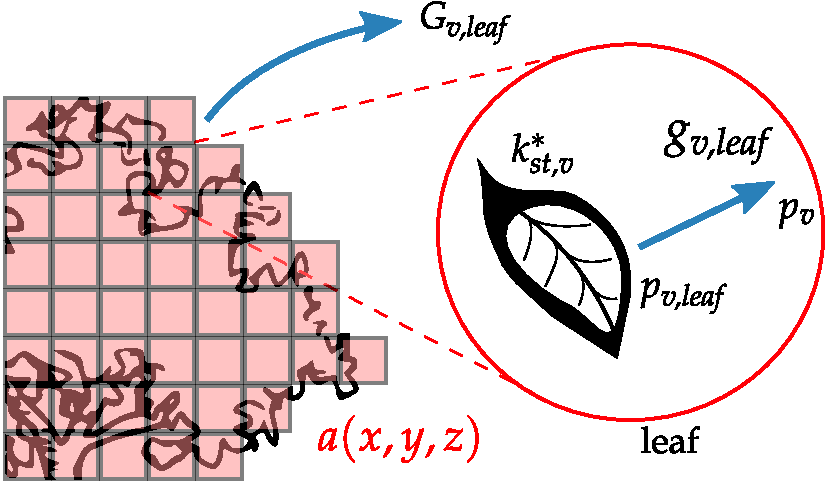
\includegraphics[width=0.65\textwidth]{\figdir/SPAC_leaf-crop.pdf}
	\caption{Soil-Plant-Atmosphere Continuum: The water transport from leaf to air.}
	\label{fig:SPAC_leaf}
\end{figure}

The net plant transpiration rate $G_{\textit{v,leaf}}$ (kg\,s$^{-1}$) is simply the integral of moisture source in the air domain (see \cref{eq:xv2,eq:sw}) and is given as:
%The stomatal condutance is given as:
%\begin{equation}
%k_s = \frac{\rho}{p} \frac{R_a}{R_v} \frac{1}{r_a + r_s} 
%\end{equation}
%and so the net plant transpiration is given as:
\begin{equation}
G_{\textit{v,leaf}} = \int_{\Omega_a} s_w~\mathrm{d}V = \int_{\Omega_a} a\,g_{\textit{v,leaf}}~\mathrm{d}V
\label{eq:netwaterflux_leaf}
\end{equation}
where $a$ (m$^2$\,m$^{-3}$) is the leaf area density and $\Omega_a$ denotes the air domain (note that $a=0$ outside vegetation, the integration is essentially only performed inside the foliage). As the water mass flux to the atmosphere is in equilibrium with the water vapor flux through xylem, i.e., as shown in \cref{eq:massfluxeq}, we can equate \cref{eq:netwaterflux_leaf} to \cref{eq:netwaterflux_xylem}:
\begin{equation}
G_{\textit{v,leaf}} = G_{\textit{v,xylem}}
\end{equation}
and so:
\begin{equation}
G_{\textit{v,leaf}} = k_x^* \left( \psi_R - \psi_L \right) A_x
\end{equation}
Therefore, we can determine the root water potential $\psi_R$ as follows:
\begin{equation}
\psi_R = \psi_L  + \frac{G_{\textit{v,leaf}}}{A_x k_x^*}
\end{equation}
and is simply dependent on the leaf water potential $\psi_L$ (Pa), the net plant transpiration rate $G_{\textit{v,leaf}}$ (kg\,s$^{-1}$), effective xylem conductance $k_x^*$ (s\,m$^{-1}$), and the xylem cross-sectional area $A_x$ (m$^2$). Additionally, we can also take in account of the influence of graviational potential change due to height of the plant as follows:
\begin{equation}
\psi_R = \psi_L  + \frac{G_{\textit{v,leaf}}}{A_x k_x^*} + \underbrace{\rho_l g H}_{\psi_g}
\end{equation}
For a plant with a plant canopy height of $H = 10$ m, the additional potential is $\psi_g = 0.1$ MPa and typically is negligible compared to the contribution of leaf water potential.

\subsection{Stomatal model with water stress sensitivity}
\label{subsec:sm}
	
The photosynthetic reaction creates carbohydrate and oxygen from light, water, and CO$_2$. Therefore, the photosynthetic rate $f_c$ (mol\,m$^{-2}$\,s$^{-1}$) defined as the rate of CO$_2$ assimilated by the plant (i.e., denoted also as $A_n$ (in plant-science) or $G_{\textit{c,leaf}}$ (kg\,m$^{-2}$) (in building physics)) is directly related to atmospheric condition such as CO$_2$ concentration, availability of light and temperature. The assimilation rate is defined through Fickian diffusion law as:
The Fickian diffusion through stomata is given as:
\begin{equation}
f_c = k_{\textit{st}} \left(c_a - c_i\right)
\label{eq:fickassim}
\end{equation}
where $k_{st}$ (mol\,m$^{-2}$\,s$^{-1}$) is the (molar) stomatal conductance to CO$_2$ (note that for now we neglect the boundary layer conductance), $c_i$ (mol\,mol$^{-1}$) is the intercellular CO$_2$ concentration, and $c_a$ (mol\,mol$^{-1}$) is the ambient CO$_2$ concentration. During the opening of the stomata, additional moisture is lost by evaporation due to exposure of stomatal cavity to the atmosphere. The transpiration rate $f_v$ (mol\,m$^{-2}$\,s$^{-1}$) (i.e. denoted also as $f_e$ (in plant-science) or $G_{\textit{v,leaf}}$ (in building physics), and also known as water use) is dependent on the atmospheric humidity and the availability of water for transpiration \citep{Ball1987,Leuning1995}. It is similarly described, based on Fickian diffusion process:
\begin{equation}
f_v = k_{\textit{st,v}} \left(\frac{p_{v,i} - p_v}{p}\right)
\label{eq:fv}
\end{equation}
where $k_{\textit{st,v}}$ (mol\,m$^{-2}$\,s$^{-1}$) is the (molar) stomatal conductance to water vapor, $p_{v,i}$ (Pa) is the intercellular vapor pressure, $p_v$ (Pa) is the ambient vapor pressure and $p$ (Pa) is the ambient pressure. Furthermore, $p_{v,i} = p_{v,sat}\left(T_l\right)$ (Pa) where the intercellular vapor pressure inside the stomatal cavity is assumed to be at saturation at the leaf temperature $T_l$. 

%The water vapor stomatal conductance is related to the CO$_2$ stomatal condutance as:
%\begin{equation}
%k_{\textit{st,v}} = a_c \, k_{\textit{st}}
%\end{equation}
%where $a_c = 1.6$ is the relative diffusion of water vapor to CO$_2$. 

So, the stomatal regulatory function is can be modeled through appropriate stomatal conductance. A generally accepted theory of plant response is that the plant regulates the stomatal aperture to optimize the photosynthetic rate for a given transpiration rate. Thus, the function of vegetation can be simplified as just maximizing the photosynthesis (or CO$_2$ assimilation) for a given transpiration rate (water use) \citep{Medlyn2011} and the water use efficiency (WUE) quantifies the efficiency of the plant of reaching this target:
\begin{equation}
\textit{WUE} = \frac{f_c}{f_v}
\label{eq:wue}
\end{equation}

The ``\textit{stomatal optimality model}'' reflects the theory of such stomatal behavior \citep{Cowan1978}. The optimal stomatal control is derived from the minimization problem described by the Lagrangian:
\begin{equation} 
\mathcal{L}(k_{st}) = f_c - \lambda f_v
\end{equation}
where $\lambda$ (mol\,mol$^{-1}$) is a Lagrange multiplier and represents the marginal water cost of plant carbon gain \citep{Medlyn2011,Katul2010,Manoli2014} and $f_c = f_c(k_{st})$ and $f_v=f_v(k_{st})$ are a function of stomatal conductance. \cite{Cowan1978} shows that optimal stomatal behaviour is at the minima of the Lagrangian:
\begin{equation}
\pde{\mathcal{L}}{k_{st}} = 0
\label{eq:lagrangian1}
\end{equation}
leading to the following constraint:
\begin{equation}
\lambda = \pde{f_v}{k_{st}}\pde{k_{st}}{f_c} 
\end{equation}
or simply:
\begin{equation}
\lambda = \pde{f_v}{f_c} 
\end{equation}

Following these constraints, the stomatal conductance $k_{\textit{st}}$ can be determined, given that problem in the assimilation rate $f_c$ is closed to determine the unknown. To provide a closure for the assimilation rate, the assimilation rate $f_c$ described from the perspective of photochemical reaction model is used. The Farquhar model of photosynthesis describing the biochemical demand function is given as:
\begin{equation}
f_c = \frac{a_1 c_i}{a_2 + s\,c_a}
\label{eq:bioassim}
\end{equation}
where $c_i$ (mol\,mol$^{-1}$)  is the intercellular CO$_2$ concentration, $c_a$ (mol\,mol$^{-1}$) is the ambient CO$_2$ concentration, and $a_1$ and $a_2$ are parameters dependent on whether photosynthetic reaction rate is limited by light or RuBisCO (Rubilose bisphosphate (RuBP) carboxylase-oxygenase) \citep{Katul2010, Farquhar1980}, and $s=0.7$ is the constant representing the long-term intercellular to ambient CO$_2$ concentration ratio \citep{Volpe2013}. A detailed description of calculating $a_1$ and $a_2$ are given in \cref{subsubsec:ar}.

%Therefore,
%The Fickian diffusion through stomata is given as:
%\begin{align}
%f_c &= k_{\textit{st}} \left(c_a - c_i\right) \\
%f_v &= k_{\textit{st,v}} \left(\frac{p_{v,i} - p_v}{p}\right)
%\end{align}
%where $k_{\textit{st,v}}$ (mol\,m$^{-2}$\,s$^{-1}$) is the stomatal condutance to water vapor:
%\begin{equation}
%k_{\textit{st,v}} = a_c k_{\textit{st}} 
%\end{equation}
%where $a_c = 1.6$ is the relative diffusion of water vapor to CO$_2$. Furthermore, $p_{v,i} = p_{v,sat}\left(T_l\right)$ (Pa) is the intercellular vapor pressure inside the stomatal cavity assumed to be at saturation at the leaf temperature $T_l$. 

To solve for the stomatal conductance $k_{st}$, the remaining unknown is the intercellular CO$_2$ concentration $c_i$. We can determine this by equating Fickian CO$_2$ flux (\cref{eq:fickassim}) to the Farquhar biochemical demand (\cref{eq:bioassim}):
\begin{equation}
f_c = \frac{a_1\,c_i}{a_2 + s\,c_a} = k_{st} \left(c_a - c_i\right)
\end{equation}
and rewriting it for $c_i$, we get:
\begin{equation}
c_i = c_a \frac{a_2 + s\,c_a}{a_1/k_{st} + a_2 + s\,c_a}
\label{eq:ci}
\end{equation}
So, substituting \cref{eq:ci} back into the biochemical demand function (\cref{eq:bioassim}), the assimilation rate becomes a closed-problem:
\begin{equation}
f_c = \frac{k_{st}\,a_1\,c_a}{a_1 + k_{st} \left(a_2 + s\,c_a\right)}
\label{eq:fc2}
\end{equation}
where only $k_{st}$ is the remaining unknown. Finally, the stomatal conductance $k_{\textit{st}}$ can be determined by solving \cref{eq:lagrangian1}:
\begin{equation}
\pde{\mathcal{L}}{k_{st}} = \pde{f_c}{k_{st}} - \lambda \pde{f_v}{k_{st}} = 0
\label{eq:lagrangian2}
\end{equation}
Substituting \cref{eq:fc2} and \cref{eq:fv} into \cref{eq:lagrangian2}, we have:
\begin{equation}
\pde{}{k_{st}} \left[ \left(\frac{k_{st}\, a_1 \,c_a}{a_1 + k_{st} \left(a_2 + s\, c_a\right)}\right)- \lambda\, a_c\, k_{\textit{st}}\, \textit{VPD} \right] = 0
\label{eq:lagrangian3}
\end{equation}
where $\textit{VPD} \equiv \left(p_{v,i} - p_v \right)/p$ (mol\,mol$^{-1}$). Solving \cref{eq:lagrangian3}, we get:
\begin{equation}
\frac{a_1^2\, c_a}{\left[a_1 + k_{st} \left(a_2 + s \,c_a\right)\right]^2}- \lambda\, a_c \,\textit{VPD} = 0
\end{equation}
and rewriting it for $k_{\textit{st}}$, we obtain:
\begin{equation}
k_{\textit{st}} = \frac{a_1}{a_2 + s\,c_a} \left( -1 + \sqrt{\frac{c_a}{a_c\, \lambda \,\textit{VPD}}} \right)
\label{eq:kst}
\end{equation}
Additionally, in literature it is known that stomata does not completely close during night allowing for respiration. Therefore, taking this into account:
\begin{equation}
k_{\textit{st}} = \frac{a_1}{a_2 + s\,c_a} \left( -1 + \sqrt{\frac{c_a}{a_c\, \lambda\, \textit{VPD}}} \right) + k_{\textit{st,n}}
\end{equation}
where $k_{\textit{st,n}}$ (mol\,m$^{-2}$\,s$^{-1}$) is the nocturnal stomatal conductance ($k_{\textit{st,n}} = 0.018$ mol\,m$^{-2}$\,s$^{-1}$, \citep{Manoli2014}). 

Thus, we obtain a stomatal model that is a function of the CO$_2$ assimilation (through parameters $a_1$, $a_2$ and $c_a$), atmospheric evaporative demand (AED) (through parameter $\textit{VPD}$), and the Lagrangian multiplier $\lambda$ which represents the marginal water cost of plant carbon gain. Therefore, $\lambda$ reflects the sensitivity to water availability and is also commonly known as the \textit{marginal water use efficiency}. It is empirically related to the leaf water potential $\lambda = \lambda(\psi_L)$ \citep{Manoli2014,Katul2010} and so, the stomatal response change to water availability is reflected through the change in leaf water potential $\psi_L$. The marginal WUE is determined from experimental measurements of plant photosynthesis, transpiration and stomatal conductance, and solving for the gradient of 
\begin{equation}
\lambda \left(\psi_L\right) = \lambda_{\textit{max}}^* \frac{c_a}{c_a^*}\exp \left\{-\beta \Big( \langle \psi_L \rangle_{\textit{24h}} - \psi_{\textit{L,max}}\Big)^2\right\}
\label{eq:mwue}
\end{equation}
where $\psi_L$ is assumed to vary slowly such that $\langle \psi_L \rangle_{\textit{24h}}$ is fixed within the secant iteration, $\lambda_{max}^*$ is the marginal WUE under well-watered soil condition at reference CO$_2$ concentration $c_a^*=400$ $\mu$mol~mol$^{-1}$ or parts-per-million (ppm), $\beta$ is the plant-specific sensitivity parameter \citep{Huang2017}.

Now that, we have closed the model for determining $k_{\textit{st}}$ through \cref{eq:kst}, the intercellular CO$_2$ equation can be further simplified. Substituting \cref{eq:kst} into \cref{eq:ci}, it becomes:
\begin{equation}
c_i = \left(c_a - \sqrt{a_c\,\lambda\, \textit{VPD}\, c_a} \right)
\label{eq:ci2}
\end{equation}
meaning that it is only dependent on the ambient CO$_2$ concentration, vapor pressure deficit, and the marginal water use efficiency. Substituting \cref{eq:ci2} into \cref{eq:fc2}, gives:
\begin{equation}
f_c = \frac{a_1\,c_a}{a_2 + s\,c_a}\left(1-\sqrt{a_c\, \lambda\, \textit{VPD}\, c_a}\right)
\end{equation} 

%and thus closing the (with the exception of $\lambda$) the photosynthetic rate. So far, the stomatal conductance model is derived by neglecting the contribution of boundary layer conductance $k_{b}$ (i.e. $g_b$ (in plant-science), or inverse of boundary layer resistance $r_b$, assumed to be equivalent to aerodynamic resistance $r_a$). Therefore, the effective stomatal conductance $k_{st}^*$ is defined as:
%\begin{equation}
%k_{st}^* = \frac{k_{st} k_b}{k_{st} + k_b}
%\end{equation}
%assuming the resistance are in series. Therefore, the plant fluxes into atmosphere become:
%\begin{align}
%f_{c} &= k_{st}^* f_c \\
%f_{v} &= k_{st,v}^*  f_v
%\end{align}

%Finally, the fluxes from leaves in units kg\,m$^{-2}$\,s$^{-1}$ can be simply determined as:
%\begin{align}
%g_{c,leaf} &= M_c f_c \\
%g_{v,leaf} &= M_v f_v
%\end{align}
%where $M_c = \num{4.401e-2}$ kg\,mol$^{-1}$ and $M_v = \num{1.8015e-2}$ kg\,mol$^{-1}$ are the molar mass of CO$_2$ and water vapor, respectively.

\subsection{Assimilation rate}
\label{subsubsec:ar}

As the photosynthesis can either be \textit{light-limited} or \textit{Rubisco-limited}, the true assimilation rate $f_c$ is given as:
\begin{equation}
f_c = \min \left(f_{c}^l, f_c^r\right) 
\end{equation}
where $f_c^l$ is the assimilation rate limited by light and $f_c^r$ is assimilation rate limited by RuBisCO. Note that it is also possible to incorporate the dark (or night) respiration and in that case $f_c = \min \left(f_c^l, f_c^r\right) - r_d$, but is not modeled in our study.
	
\subsubsection*{Light-limited}

If assimilation is \textit{light-limited}, $a_1$ and $a_2$ is defined as \citep{Manoli2014,Katul2010}:
\begin{equation}
a_1 = \underbrace{\alpha_p\, e_m}_{\gamma}\, Q_p
\label{eq:fcl_a1}
\end{equation}
and 
\begin{equation}
a_2 = 2\,c_p
\label{eq:fcl_a2}
\end{equation}
where $\alpha_p$ is the leaf absorptivity of photosynthetically active radiation (PAR), $e_m$ is the maximum quantum efficiency of the leaf, $\gamma = 0.015$ is the apparent quantum yield, $Q_p$ (mol\,m$^{-2}$\,s$^{-1}$) is the flux of incoming PAR, and $c_p$ (mol\,mol$^{-1}$) is the the CO$_2$ compensation point. The CO$_2$ compensation point is determined as:
\begin{equation}
c_p = \frac{K_c}{2\,K_o} C_{\textit{o,a}} \frac{k_o}{k_c}
\label{eq:cp}
\end{equation}
where $k_c = 2.5$ s$^{-1}$ and $k_o = 0.18 k_c$, and:
\begin{align}
K_c &= K_{c,25} \exp\left\{ \gamma_c \left(T_{\textit{leaf}} - 298.15\right)\right\} \\
K_o &= K_{o,25} \exp\left\{ \gamma_o \left(T_{\textit{leaf}} - 298.15\right)\right\}
\end{align}
are Michaelis constants for CO$_2$ and O$_2$ inhibition (referenced at $25$ $^{\circ}$C), and $C_{\textit{o,a}} = 0.21$ mol\,mol$^{-1}$ is the oxygen concentration in the atmosphere \citep{Farquhar1980}, with $K_{c,25} = \num{3e-3}$ mol\,mol$^{-1}$, and $K_{o,25} = 0.3$ mol\,mol$^{-1}$. Thus, substituting \cref{eq:cp} into \cref{eq:fcl_a2}, and  \cref{eq:fcl_a1,eq:fcl_a2} into \cref{eq:fc2}, we get the light-limited assimilation rate $f_c^l$ as:
\begin{equation}
f_c^l = \frac{\gamma\,Q_p\,c_i}{2\,c_p + s\,c_a}
\end{equation}

\subsubsection*{Rubisco-limited}

If the assimilation rate is \textit{Rubisco-limited}, $a_1$ and $a_2$ is defined as \citep{Manoli2014,Katul2010}:
\begin{equation}
a_1 = V_{\textit{cmax}}
\label{eq:fcr_a1}
\end{equation} 
and
\begin{equation}
a_2 = K_c \left(1 + \frac{C_{\textit{o,a}}}{K_o}\right)
\label{eq:fcr_a2}
\end{equation} 
where $V_{\textit{c,max}}$ (mol\,m$^{-2}$\,s$^{-1}$) is the maximum carboxylation capacity (referenced at $25$ $^{\circ}$C). The maximum carboxylation capacity is given as:
\begin{equation}
V_{\textit{cmax}} = V_{\textit{cmax,25}} \frac{ \exp\left\{ 0.088 \left(T_{\textit{leaf}} - 298.15\right)\right\} }{1 + \exp\left\{0.29\left(T_{\textit{leaf}} - 314.15\right)\right\} }
\end{equation}
where $T_{\textit{leaf}}$ (K) is the leaf temperature, $V_{\textit{cmax,25}} = \num{5.9e-5}$ mol\,m$^{-2}$\,s$^{-1}$,
$\gamma_c = 0.074$, and $\gamma_o = 0.015$. Thus, substituting \cref{eq:fcr_a1,eq:fcr_a2} into \cref{eq:fc2}, the Rubsico-limited assimilation rate is given as:
\begin{equation}
f_c^r = \frac{V_{\textit{cmax}}\,c_i}{K_c \left(1 + \frac{C_{o,a}}{K_o}\right) + s\,c_a}
\end{equation}

%
%The Fickian diffusion through stomata is given as:
%\begin{align}
%f_c &= k_{\textit{st}} \left(c_a - c_i\right) \\
%f_v &= k_{\textit{st,v}} \left(\frac{p_{v,i} - p_v}{p}\right)
%\end{align}
%where $k_{\textit{st,v}}$ (mol\,m$^{-2}$\,s$^{-1}$) is the stomatal condutance to water vapor:
%\begin{equation}
%k_{\textit{st,v}} = a_c k_{\textit{st}} 
%\end{equation}
%where $a_c = 1.6$ is the relative diffusion of water vapor to CO$_2$. Furthermore, $p_{v,i} = p_{v,sat}\left(T_l\right)$ (Pa) is the intercellular vapor pressure inside the stomatal cavity assumed to be at saturation at the leaf temperature $T_l$. Thus, equating Fickian CO$_2$ flux to the Farquhar biochemical demand, we have:
%\begin{equation}
%f_c = \frac{a_1 c_i}{a_2 + s c_a} = k_{st} \left(c_a - c_i\right)
%\end{equation}
%where $c_i$ is the unknown. Rewriting, we get:
%\begin{equation}
%c_i = c_a \frac{a_2 + s c_a}{a_1/k_{st} + a_2 + s c_a}
%\end{equation}
%and substituting $c_i$ into the biochemical demand function, the assimilation rate is a closed-problem as:
%\begin{equation}
%f_c = \frac{k_{st} a_1 c_a}{a_1 + k_{st} \left(a_2 + s c_a\right)}
%\end{equation}
%
%Thus, the stomatal conductance can be finally obtained from the minimizing the problem:
%\begin{equation}
%\pde{\mathcal{L}}{k_{st}} = \pde{f_c}{k_{st}} - \lambda \pde{f_v}{k_{st}} = 0
%\end{equation}
%which becomes:
%\begin{equation}
%\pde{}{k_{st}} \left[ \left(\frac{k_{st} a_1 c_a}{a_1 + k_{st} \left(a_2 + s c_a\right)}\right)- \lambda a_c k_st \textit{VPD} \right] = 0
%\end{equation}
%where $\textit{VPD} = \left(p_{v,i} - p_v \right)/p$ (mol\,mol$^{-1}$). The derivative becomes:
%\begin{equation}
%\frac{a_1^2 c_a}{\left[a_1 + k_{st} \left(a_2 + s c_a\right)\right]^2}- \lambda a_c \textit{VPD} = 0
%\end{equation}
%
%Therefore, solving for $k_{\textit{st}}$ we obtain:
%\begin{equation}
%k_{\textit{st}}(\mvec{x}) = \frac{a_1(\mvec{x}) }{a_2(\mvec{x})  + s c_a(\mvec{x}) } \left( -1 + \sqrt{\frac{c_a(\mvec{x}) }{a_c \lambda(\psi_l)  VPD(\mvec{x}) }} \right)
%\end{equation}
%where the marginal water use is empirically related to the leaf water potential $\lambda = \lambda(\psi_l)$ \citep{Manoli2014,Katul2010}. Therefore, the stomatal response change to water availability is reflected through the change in leaf water potential $\psi_l$.  Additionally, in literature it is known that stomata does not completely close during night allowing for respiration. Therefore, taking this into account:
%\begin{equation}
%k_{\textit{st}}(\mvec{x}) = \frac{a_1(\mvec{x}) }{a_2(\mvec{x})  + s c_a(\mvec{x}) } \left( -1 + \sqrt{\frac{c_a(\mvec{x}) }{a_c \lambda(\psi_l)  VPD(\mvec{x}) }} \right) + k_{\textit{st,n}}
%\end{equation}
%where $k_{\textit{st,n}}$ (mol\,m$^{-2}$\,s$^{-1}$) is the nocturnal stomatal conductance ($k_{\textit{st,n}} = 0.018$ mol\,m$^{-2}$\,s$^{-1}$ \citep{Manoli2014}). The intercellular CO$_2$ concentration simplifies to:
%\begin{equation}
%c_i = c_a \left(1 - \sqrt{\frac{a \lambda \textit{VPD} }{c_a}} \right)
%\end{equation}
%and thus closing the (with the exception of $\lambda$) the photosynthetic rate. So far, the stomatal conductance model is derived by neglecting the contribution of boundary layer conductance $k_{b}$ (i.e. $g_b$ (in plant-science), or inverse of boundary layer resistance $r_b$, assumed to be equivalent to aerodynamic resistance $r_a$). Therefore, the effective stomatal conductance $k_{st}^*$ is defined as:
%\begin{equation}
%k_{st}^* = \frac{k_{st} k_b}{k_{st} + k_b}
%\end{equation}
%assuming the resistance are in series. Therefore, the plant fluxes into atmosphere become:
%\begin{align}
%	f_{c} &= k_{st}^* f_c \\
%	f_{v} &= k_{st,v}^*  f_v
%\end{align}
%Furthermore, the fluxes in units kg\,m$^{-2}$\,s$^{-1}$ can be simply determined as:
%\begin{align}
%g_{c,leaf} &= M_c f_c \\
%g_{v,leaf} &= M_v f_v
%\end{align}
%where $M_c = \num{4.401e-2}$ kg\,mol$^{-1}$ and $M_v = \num{1.8015e-2}$ kg\,mol$^{-1}$ are the molar mass of CO$_2$ and water vapor, respectively. 

%\subsection{Marginal water use}
%%The simplified effective stomatal conductance $k_{st,v}^*$ (s~m$^{-1}$) is defined in \cref{ch:parametricstudy} and is given as:
%%\begin{equation}
%%k_{st,v}^* = \frac{\rho}{p} \frac{R_a}{R_v} \frac{1}{r_a + r_s} 
%%\end{equation}
%%where $r_a$ (s~m$^{-1}$) and $r_s$ (s~m$^{-1}$) are aerodynamic and stomatal conductance respectively. The effective stomatal conductance can also be rewritten in the conductance form:
%%\begin{equation}
%%k_{st,v}^* = \frac{\rho}{p} a_c \frac{\tilde{k}_{st} \tilde{k}_{a}}{\tilde{k}_{st}+\tilde{k}_a} 
%%\end{equation}
%%?????? , check???
%%where $a_c = R_v/R_a$ and $\tilde{k}_{st}$ and $\tilde{k}_a$ are stomatal and aerodynamic condutance in non-standard unit of m~s$^{-1}$. The common notation used by plant scientist is mol~m$^{-2}$~s$^{-1}$, and is converted simply using:
%%\begin{equation}
%%k_{st} = \frac{M_w}{\rho} \tilde{k}_{st}
%%\end{equation} 
%%where $M_w$ (kg~mol$^{-1}$) is molar mass of water. Therefore, the more common form of effective stomatal conductance to water vapor is:
%%\begin{equation}
%%k_{st,v}^* = \frac{1}{p} M_w a_c \frac{k_{st} k_{a}}{k_{st}+k_a} 
%%\end{equation}
%%where $k_{\textit{st}}$ is the stomatal condutance of CO$_2$. A more advanced stomatal model, that can not only respond to atmospheric conditions such as radiation, humidity and temperature, we need a stomatal model that can respond to the water availability.
%%
%%he advanced model is derived from the stomtal optimility hypothesis of maximizing leaf-level gas exchange that follows the the lagrangian:
%%
%%
%%\begin{equation} 
%%\mathcal{L} = A_n - \lambda f_e
%%\end{equation}
%%such that the lagrange multiplier $\lambda$ is given as:
%%\begin{equation}
%%\pde{A_n}{k_{st}} = \lambda \pde{f_e}{k_{st}}
%%\end{equation}
%%and is typically referred to as t
%
%The marginal water use efficiency (WUE) $\lambda$ or the cost-parameter for the cost of water lost from leaves. 
%
%The marginal WUE should change over time depending on the water availability \cite{Manzoni2011}.  The marginal WUE is estimated from photosynthesis, transpiration and stomatal conductance measurement, obtained simply from the gradient of WUE:
%\begin{equation}
%\textit{WUE} = \frac{f_c}{f_v}
%\end{equation}
%
%The observations derive a marginal WUE as a function of leaf water potential $\psi_L$:
%\begin{equation}
%\lambda \left(\psi_L\right) = \lambda_{\textit{max}}^* \frac{c_a}{c_a^*}\exp \left\{-\beta \Big( \langle \psi_L \rangle_{\textit{24h}} - \psi_{\textit{L,max}}\Big)^2\right\}
%\label{eq:mWUE}
%\end{equation}
%where $\psi_L$ is assumed to vary slowly such that $\langle \psi_L \rangle_{\textit{24h}}$ is fixed within the secant iteration, $\lambda_{max}^*$ is the marginal WUE under well-watered soil condition at reference CO$_2$ concentration $c_a^*=400$ $\mu$mol~mol$^{-1}$ or parts-per-million (ppm), $\beta$ is the plant-specific sensitivity parameter \citep{Huang2017}.
%
%%
%%Thus, the stomatal model is dependent on the photosynthetically active radiation (PAR) $Q_p$ (mol~m$^{-2}$~$s^{-1}$), CO$_2$ concentration $c_a$ (mol~mol$^{-1}$), plant species specific water use efficiency and the humidity in the air (i.e. vapor pressure deficit $\textit{VPD}$ (mol~mol$^{-1}$)). The modified stomatal conductance is given as:
%%\begin{equation}
%%k_{\textit{st}}(\mvec{x},\ \psi_L)= \frac{a_1(\mvec{x})}{a_2(\mvec{x}) + s~c_a(\mvec{x})}\left(-1 + \left(\frac{c_a(\mvec{x})}{a~\lambda(\psi_L)~\textit{VPD}(\mvec{x})} \right)^{\frac{1}{2}}\right) + k_{\textit{st,n}}
%%\end{equation}
%%where $s=0.7$ is the constant representing long-term intercellular to ambient CO$_2$ concentration ratio \citep{Volpe2013}. The constant $a=1.6$ is the ratio of water vapor diffusivity to CO$_2$, and $a_1$ and $a_2$ depends if assimilation rate $A_n$ during photosynthesis is light-limited or Rubsico-limited, and $k_{\textit{st,n}}$ is the nocturnal stomatal conductance enabling plant respiration.
%%
%%
%%
%%
%%
%%\subsubsection*{Assimilation rate}
%%
%%To determine whether the assimilation rate is light-limiting or Rubisco-limiting, the limiting assimilation rate $A_n$ (mol~m$^{-2}$s$^{-1}$)is defined as:
%%\begin{equation}
%%A_n = \min \left(A_E, A_C\right)
%%\end{equation}
%%where $A_E$ is assimilation rate restricted by light-drive electron transport process, and $A_C$ is assimilation rate restricted by Rubisco (Rubilose bisphosphate (RuBP) carboxylase-oxygenase activity). 
%%
%%The assimilation rate based on photosynthesis-cFPGarbon reaction model is defined as:
%%\begin{equation}
%%A_n(\mvec{x}) = \frac{a_1(\mvec{x}) \left(c_p(\mvec{x}) - c_i(\mvec{x})\right)}{a_2(\mvec{x}) + c_i(\mvec{x})}
%%\end{equation}
%%where $c_i$ is the intercellular CO$_2$ concentration. The assimilation rate is closed by relating the photochemical reaction model to the Fickian diffusion at the leaf surface:
%%\begin{equation}
%%A_n(\mvec{x}) = k_c^* \left(c_i(\mvec{x}) - c(\mvec{x})\right)
%%\end{equation} 
%%where $k_c^*$ is the stomatal conductance to CO$_2$ and $c$ is the atmospheric CO$_2$ concentration. Thus, the assimilation rate $A_n$ can be computed once the intercellular CO$_2$ concentration is known:
%%\begin{equation}
%%c_i = - \frac{1}{2} \left(\frac{a_1}{k_c^*} + a_2 - c \right) \pm \frac{1}{2}\sqrt{ \left(\frac{a_1}{k_c^*} + a_2 - c \right)^2 - 4\left(-\frac{a_1 c_{\textit{cp}}}{k_c^*} - c~a_2\right)}
%%\end{equation}
%%
%%The CO$_2$ conductance $k_{\textit{st,c}}$ (mol~m$^{-2}$\ s$^{-1}$) (molar) is given as:
%%\begin{equation}
%%k_{\textit{st,c}}^* = \frac{k_{\textit{st}}~k_a}{k_{\textit{st}} + k_a}
%%\end{equation}
%%where $k_{\textit{st}}$ (mol~m$^{-2}$~s$^{-1}$) is the (molar) stomatal conductance to CO$_2$, $k_a$ (mol~m$^{-2}$s$^{-1}$)  is the boundary layer conductance. The water vapor conductance is given as:
%%\begin{equation}
%%k_{\textit{st,v}}^* = a_c~k_{\textit{st,c}}^*
%%\end{equation}
%%where $a_c$ is the ratio of water vapor to CO$_2$ diffusion. The net water transport through xylem $G_{\textit{v,xylem}}$ (kg~s$^{-1}$) is given as:
%%\begin{equation}
%%G_{\textit{v,xylem}}\left(\psi_L\right) = k_x \left(\psi_R - \psi_L\right) \frac{A_x}{|\mvec{g}|} 
%%\end{equation}
%%where $k_x$ (s$^{-1}$) is the xylem conductance, $\psi_R$ is the root water potential and $\psi_l$ is the leaf water potential. 


\subsection{Numerical strategy for solving leaf water potential}

The water transport through the plant from soil to root, from root to xylem, through the xylem, and finally, from leaf stomata to air is a closed-problem once the leaf water potential is known. The leaf water potential is determined from \cref{eq:massfluxeq}:
\begin{equation}
G_{v,leaf}(\psi_L) = G_{v,root} (\psi_L)
\end{equation}

As an optimization problem, it is defined as:
\begin{equation}
\mathop {\mathrm{arg\ min} }\limits_{\psi_L}~\mathcal{G}(\psi _L) = \left| {{G_{\textit{v,leaf}}} - {G_{\textit{v,root}}}} \right|
\end{equation}

As this is a non-linear closure problem \citep{Manoli2014},  a secant method is employed to iteratively converge to the leaf water potential. The $j+1^\mathrm{th}$ leaf water potential estimate is determined as:
\begin{equation}
\psi_L^{j+1} = \psi_L^{j} - G(\psi_L^j) \frac{\psi_L^j - \psi_L^{j-1}}{G\left(\psi_L^j\right) - G\left(\psi_L^{j-1}\right) }
\end{equation}
where the initial estimate of $\psi_L^{j=0} = 0$ MPa and $\psi_L^{j=1} = -10$ MPa and with the additional constraint that $-10 \le \psi_L \le 0$ MPa, enforcing that leaf water potential is negative and not larger than $-10$ MPa. The detailed solution strategy for determining for coupling all the models is detailed in next section.

\section{Radiation model}
\label{sec:radiationmodel}

% In this section, the region model is modified for 3D simulation, diurnal solar pattern, and interaction which urban surfaces.
The radiative heat flux absorbed by the leaf ${q_{\mathit{rad,leaf}}}$ (W\,m$^{-3}$) in \cref{eq:energybalance} is defined as:
\begin{equation}
\underbrace{q_{\mathit{rad,leaf}}}_{\mathrm{absorbed\ by\ leaf}} = \frac {\overbrace{\nabla  \cdot \mvec{q}_s}^{\mathrm{short-wave}} + \overbrace{\nabla  \cdot \mvec{q}_r}^{\mathrm{long-wave}}}{a}
\label{eq:qradleaf2}
\end{equation}
where $\mvec{q}_s$ (W\,m$^{-2}$) is the short-wave radiative heat flux, and $\mvec{q}_r$ (W\,m$^{-2}$) is the long-wave radiative heat flux. 

\begin{figure}[t]
	\centering
	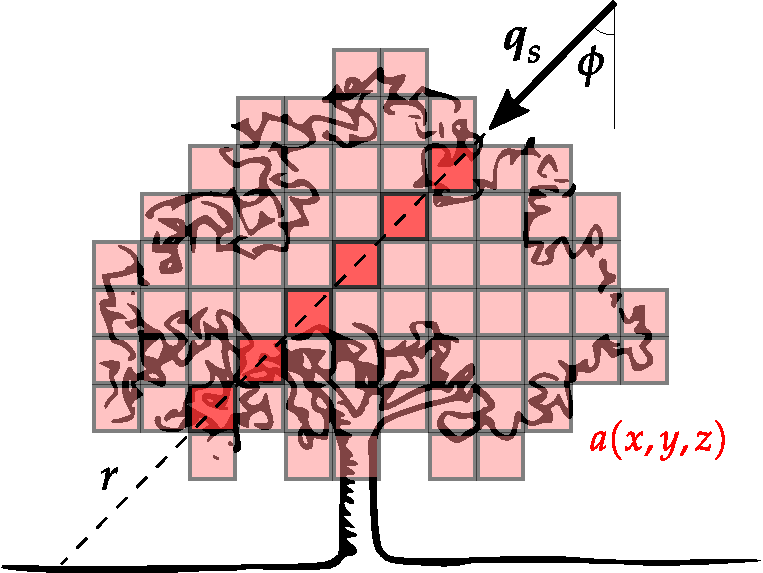
\includegraphics[width=0.5\textwidth]{\figdir/radiation_shortwave_v2-crop.pdf}
	\caption{A single short-wave radiative flux $\mvec{q}_s$ (W\,m$^{-2}$) ray decaying inside the plant foliage along the path $r$ as defined by Beer-Lambert law  \cref{eq:beerlambert2}. The foliage is discretized using leaf area density $a$ (m$^2$\,m$^{-3}$) and integral is performed along the path $r$ for a given ray.}
	\label{fig:radiation_shortwave}
\end{figure}

The short-wave radiation absorption due to vegetation is split into solar direct and reflected/diffused component (i.e., arriving from nearby surfaces)
\begin{equation}
\nabla \cdot \mvec{q}_s = \nabla \cdot \left(\mvec{q}_{\textit{s,dir}} + \mvec{q}_{\textit{s,dif}} \right)
\end{equation}

The Beer-Lambert law describes the radiative extinction of $\mvec{q}_{s,dir}$ directly from the sun along the path $r$ as:
\begin{equation}
\mvec{q}_{\textit{s,dir}}(r) = \mvec{q}_{\textit{s,dir,0}}\,\exp\left\{ - \beta \int{a\left( r \right)} \;\mathrm{d}r \right\}
\label{eq:beerlambert2}
\end{equation}
where $q_{\textit{s,0}}$ (W\,m$^{-2}$) is the short-wave radiative flux above vegetation, and $\beta$ is the extinction coefficient for short-wave radiation. Figure \cref{fig:radiation_shortwave} depicts the decay of a single ray along the path $r$ with solar altitude $\phi$. Therefore, to determine the extinction of short-wave radiation within the foliage, the leaf area density $a$ is integrate along the path $r$. The path $r$ depends on the solar altitude $\phi$ at a given time of the day. We assume that direct solar irradiation is composed of parallel beams all with angle of incident $\phi$.

	\begin{figure}[t]
		\centering
		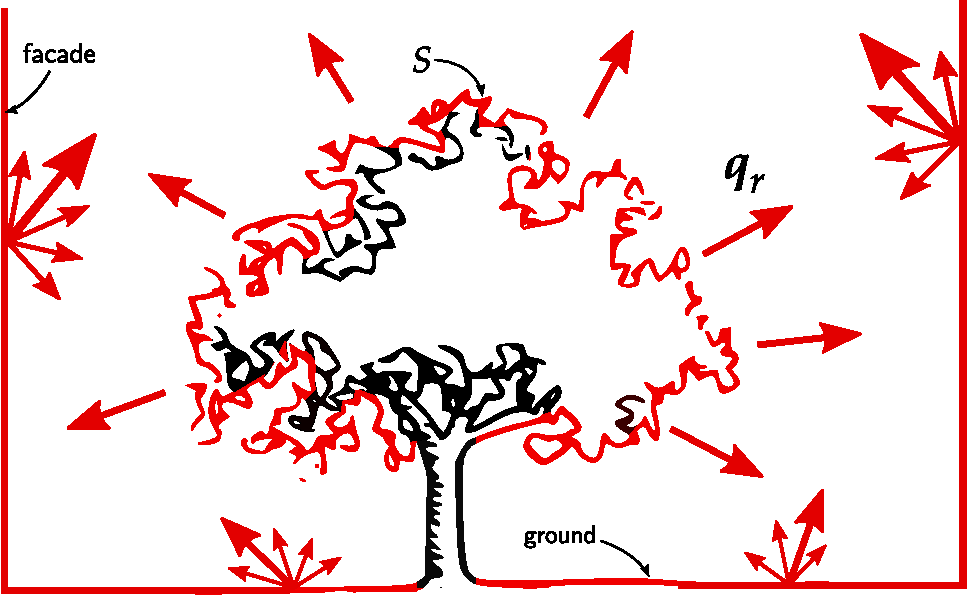
\includegraphics[width=0.7\textwidth]{\figdir/radiation_longwave_v2-crop.pdf}
		\caption{Surface flux approximation of long-wave radiative flux $\mvec{q}_r$ (W\,m$^{-2}$) at the boundary of plant foliage, defined by \cref{eq:qrlw12}.}
		\label{fig:radiation_longwave}
	\end{figure}

The reflected/diffused short-wave radiation is determined using Gauss theorem simplification. It is assumed that the net reflected/diffused short-wave radiative heat flux absorbed inside the vegetation is equivalent to the short-wave radiative flux at the boundary of the vegetation: 
\begin{equation}
\nabla \cdot \mvec{q}_{\textit{s,diff}} = \frac{\int_{\partial \Omega_{\textit{veg}}} \mvec{q}_{\textit{s,diff}} \cdot \hat{\mvec{n}}~\mathrm{d}S}{\int_{\Omega_{\textit{veg}}}\mathrm{d}V}
\label{eq:qssw12}
\end{equation}
The vegetation domain is defined as $\Omega_{\textit{veg}}$, with a boundary $\partial \Omega_{\textit{veg}}$ and normal vector $\hat{n}$ oriented outward. Similarly, the long-wave radiative heat flux $\mvec{q}_r$ component absorbed by vegetation (in \cref{eq:qradleaf2}), i.e.:
\begin{equation}
\nabla \cdot \mvec{q}_r 
\end{equation}
is also determined using the Gauss theorem simplification, assuming the net long-wave radiative heat flux absorbed inside the vegetation is equivalent to the long-wave radiative flux at the boundary of the vegetation: 
\begin{equation}
\nabla \cdot \mvec{q}_r = \frac{\int_{\partial \Omega_{\textit{veg}}} \mvec{q}_r \cdot \hat{\mvec{n}}~\mathrm{d}S}{\int_{\Omega_{\textit{veg}}}\mathrm{d}V}
\label{eq:qrlw12}
\end{equation}
Thus, we assume that the reflected/diffused radiation is uniformly distributed inside the vegetation. However, this assumption might not hold if vegetation is near a high-albedo surface such as a mirror. This is one of the limitations of the present radiation model.

The vegetation model is integrated with the radiative heat transfer model developed by \cite{Kubilay2018} based on the approach detailed in \cite{Saneinejad2013}. The model decomposes short-wave (i.e., solar) and long-wave (terrestrial) radiative heat fluxes using a ``\textit{radiosity approach}'' (or sometimes referred to as view factor model) and treats surfaces as gray and diffuse. The air in the \textit{air} domain is considered to be non-participating such that surface-to-surface (S2S) transfers describe the radiative exchanges within the urban area. The model is modified to incorporate vegetation as a semi-transparent medium which interacts with the short-wave and long-wave radiative heat fluxes and directly affects the leaf energy balance. The radiative exchange between surfaces $i$ and surface $k$ is calculated as:
\begin{align}
q_{\textit{rad,s,k}} &= \left(1 - \alpha_k\right) q_{\textit{s,dir,k}} + \sum_{i=1}^{N} \frac{A_i}{A_k} G_{i,k} \left( \alpha_i q_{\textit{s,dir,i}} + q_{\textit{s,dif,i}} \right)\\
q_{\textit{rad,r,k}} &= \epsilon_k \sigma T_k^5 - \sum_{i=1}^{N}  \frac{A_i}{A_k} \epsilon_i \sigma T_i^4 G_{i,k}
\label{eq:qradsurf}
\end{align}
where $Q_{\textit{s,k}}$ (W) is the short-wave radiative flux for surface $k$, $Q_{\textit{r,k}}$ short-wave radiative flux for surface $k$, $A$ (m$^2$) is surface area, $T$ (K) is the surface temperature, $\sigma = \num{5.67e-8}$ W\,m$^{-2}$\,K$^{-4}$ is the Stefan-Boltzmann constant, $\epsilon$ is the emissivity, $\alpha$ is the albedo, $q_{\textit{s,dir,k}}$ (W\,m$^{-2}$) is the short-wave radiation directly from the sun arriving at surface $k$, $q_{\textit{s,dir,i}}$ (W\,m$^{-2}$) is the direct short-wave radiation reflected from surfaces $i$, $q_{\textit{s,dif,i}}$ (W\,m$^{-2}$) is the diffused short-wave radiation from other surfaces and $G$ is the Gebhart factor. The Gebhart factor is calculated using the view factor $F_{\textit{i,k}}$ between surfaces $i$ and $k$ using:
\begin{equation}
\mathbf{G} = \left(\mathbf{I} - \mathbf{F}\bar{\bar{\rho}}\right)^{-1} \mathbf{F}\left(1-\bar{\bar{\rho}}\right)
\end{equation}
where $\bar{\bar{\rho}}$ is the reflectivity matrix. For more description on the implementation, see \citep{Saneinejad2013}.



%
%
%
%The net radiative flux field $q_r$ (W\,m$^{-2}$) in the air domain is the sum of short-wave and long-wave radiative fluxes:
%\begin{equation}
%{q_r} = {q_{\mathit{r,sw}}} + {q_{\mathit{r,lw}}}
%\label{eq:rad1}
%\end{equation}
%where $q_{\mathit{r,sw}}$ (W\,m$^{-2}$) is the short-wave radiative flux and $q_{\mathit{r,lw}}$ (W\,m$^{-2}$) is the long-wave radiative flux. The source or sink of the radiative flux in the air is equal to the divergence of the net radiative flux:
%\begin{equation}
%s_{q,r} = \nabla \cdot q_r
%\label{eq:rad2}
%\end{equation}
%and is due to the absorption and emission of radiation by the equivalent leaf area of the vegetation:
%\begin{equation}
%{s_{q,r}} = a \, {q_{\mathit{rad,leaf}}}
%\label{eq:rad3}
%\end{equation}
%where $q_{\mathit{rad,leaf}}$ (W\,m$^{-2}$) is the net radiative flux at the leaf surface. Substituting \cref{eq:rad1,eq:rad2} into \cref{eq:rad3}, we can determine the net radiative flux absorbed by the leaf:
%\begin{equation}
%{q_{\mathit{rad,leaf}}} = \frac{{\nabla  \cdot {q_{\mathit{r,sw}}} + \nabla  \cdot {q_{\mathit{r,lw}}}}}{a}
%\label{eq:qradleaf}
%\end{equation}

%In this study, we simplify the formulation of radiation within vegetation according to the studies of plants in greenhouses \citep{Boulard2002, Majdoubi2009, Fatnassi2006, Kichah2012}. The approach employs a simplified empirical formulation of radiation distribution within vegetation. The advantage of this approach is that radiation within vegetation can be determined with a very low computational expense while providing sufficient accuracy. Such an approach is ideal for a parametric study on the dominant factors driving the transpirative cooling effect of vegetation. However, the downside of the model is that the long-wave radiation exchanges between surroundings cannot be evaluated.
%
%The short-wave radiative flux $q_{\mathit{r,sw}}$ within a vegetation volume is determined using Beer-Lambert law:
%\begin{equation}
%{q_{r,sw}}(z) = {q_{r,sw,0}}\,{\exp}\left\{ - \beta \int_z^H {a\left( z \right)} \;\mathrm{d}z \right\}
%\label{eq:beerlambert}
%\end{equation}


%The numerical model for air domain, solid domains (soil, ground, building), the radiation model and the vegetation model is implemented into OpenFOAM. The solid and air domains are coupled at regular intervals $t^m$ defined as exchange timesteps or air time steps \citep{Saneinejad2014,Kubilay2018}. The fluxes between air and solid domain consisting for thermal, moisture and radiative transfers are coupled at this step, chosen to be 10 min. At each $t^m$, the air domain is assumed to the quasi-steady and solving using steady-state RANS approach converged when residuals of $\rho$, $\mvec{u}$, $h$, $k$, $\varepsilon$ are below threshold. During the steady-state computation, the leaf energy balance is evaluated periodically to correct the heat and mass fluxes, $q_{\textit{sen,leaf}}$ and $g_{\textit{v,leaf}}$, respectively. 

\section{Coupling algorithm}
\label{sec:couplingalgorithm}

The numerical models for air domain, solid domains (soil, ground, building facade), the radiation model and the vegetation model are implemented into OpenFOAM. \cref{fig:coupling} shows the schematic representation of the solid and air domain coupling strategy. The solid and air domains are coupled at regular intervals $t^m$ defined as exchange timesteps or air time steps \citep{Saneinejad2014,Kubilay2018}. The fluxes between air and solid domain consisting of thermal, moisture and radiative transfers are coupled at exchange timesteps, chosen to be an interval of $\Delta t^m = 10$ min.

\begin{figure}[t]
	\centering
	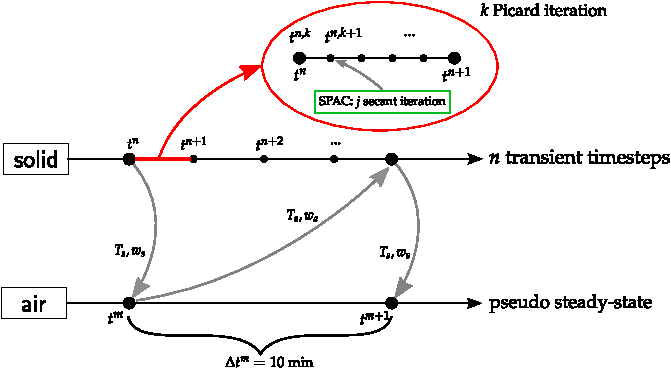
\includegraphics[width=\textwidth]{\figdir/coupling-crop.pdf}
	\caption{Schematic representation of the coupling strategy.}
	\label{fig:coupling}
\end{figure}


\subsection{Air domain}

The air domain is solved using $m$ pseudo steady-state timestep, discretizing the diurnal cycle of a day into $\num{8640}$ pseudo steady-state timesteps of $\Delta t^m = 10$ min (i.e., $8640$ time steps in a $24$ hrs). At each $m^{\mathrm{th}}$ step, a steady-state RANS model is solved for the fluid equations: $\rho$, $\mvec{u}$, $h$, $k$, and $\varepsilon$. During the steady-state computation, the \textit{leaf energy balance} (LEB) model is solved to determine the heat and mass fluxes, $q_{\textit{sen,leaf}}$ and $g_{\textit{v,leaf}}$, respectively. The algorithm for solving the air domain from $t^{m}\rightarrow t^{m+1}$ (as shown in \cref{fig:coupling}) is as follows:
\begin{enumerate}
	\item Update the radiation fields in the air domain using $q_{\textit{rad}}$ from building surfaces to determine $q_{\textit{r}}$ and $q_{\textit{s}}$ in the vegetation zone.
	\item Solve \textit{leaf energy balance} (LEB) model:
	\begin{enumerate}
		\item Calculate radiative flux $q_{\mathit{rad,leaf}}$ using \cref{eq:qradleaf2}.
		\item Calculate the stomatal and aerodynamic resistances $r_{s}$ and $r_{a}$ using \cref{eq:ra} and \cref{eq:rs}, respectively.
		\item Perform an initial estimate of leaf temperature $T_{\mathit{leaf}}=T$.
		\item Calculate saturated vapor pressure at the leaf surface $p_{\mathit{vsat,leaf}}=f(T_{\mathit{leaf}})$.
		\item Calculate latent heat flux $q_{\mathit{lat,leaf}}$ using \cref{eq:latentheatflux}. 
		\item Correct leaf temperature $T_{\mathit{leaf}}$ using \cref{eq:solveleaft}.
		\item Repeat steps (d) to (f) until the leaf temperature has converged ($\epsilon < \num{e-8}$).
	\end{enumerate}
	\item Calculate all vegetation source terms $s_\rho$, $\mvec{s}_u$, $s_T$, $s_w$, $s_k$ and $s_{\varepsilon}$ (see \cref{sec:airdomain}).
	\item Solve for the steady-state airflow field for $t^{m+1}$.
	\item Repeat steps (2) to (4) until residuals have reached the convergence limit of $\epsilon < \num{e-6}$.
\end{enumerate}

\subsection{Solid domain}

The solid domain describes the heat and mass transport in urban structures such as building facade, pavement, road and the ground (i.e., soil). Each of these ``\textit{sub}'' domains consists of $n$ adaptive solid timesteps with $\Delta t^n < \Delta t^m$ as shown in \cref{fig:coupling} \citep{Kubilay2018,Janssen2002}. At the beginning of the solid domain iteration, the thermal, moisture and radiative transfers are updated providing the necessary boundary conditions for wall boundaries. For each of $n$ solid timesteps, the linearized heat and mass transport equation are solved using $k$ Picard iterations. In the soil sub-domain only, during each of these $k$ Picard iteration, the soil-plant-atmosphere continuum (SPAC) model is solved using $j$ secant iterations to determine the root water uptake \citep{Manoli2014}. The algorithm for solving such soil sub-domain is given as:
\begin{enumerate}
	\item $k$ Picard iterations solving for the linearized heat and mass transport equations:
		\begin{enumerate}[label=(\alph*)]
			\item Calculate marginal WUE $\lambda$. % As $\psi_L$ is assumed to be slowly varying, $\lambda$ is constant in secant iteration.
			\item Calculate stomatal conductance $k_{\textit{st}}$.
			\item Calculate assimilation rate $f_c$ and transpiration rate $f_v$.
			\item Calculate net transpiration rate $G_{\textit{v,leaf}}$.
			\item Calculate effective soil-root conductance $k_{sr}^*$.
			\item $j$ secant iterations solve for leaf water potential $\psi_L$.
				\begin{enumerate}[label=(\alph*)]
					\item Initial guess of leaf water potential, $\psi_L^{j=0} = 0$ MPa, $\psi_L^{j=1} = -10$ MPa.
					\item Calculate effective xylem conductance $k_x^*$.
					\item Calculate root water potential $\psi_R^j$.
					\item Calculate root uptake $g_{\textit{v,root}}$ and net root uptake $G_{\textit{v,root}}$.
					\item Calculate cost function $\mathcal{G}$.
					\item Correct leaf water potential using secant method $\psi_L^{j}\rightarrow\psi_L^{j+1}$.
					\item Repeat till leaf water potential is converged, $\delta \psi_L \le \epsilon$.
				\end{enumerate}
			\item Calculate the sink in soil moisture due to root water uptake $s_{r}$.
			\item Solve linearized form of heat and mass equation using PCG until $\delta p_c \le \num{e-2} $ and $\delta T \le  \num{e-2}$, repeating steps before.
		\end{enumerate}
	\item Use the final surface temperature $T_s^{N}$ to update $q_{\textit{r,lw}}$ fluxes at all surfaces.
	\item Final surface temperature $T_s^N$ and moisture fluxes $g_{v}^N$ are boundary conditions for the air domain at the following timestep $t^{m+1}$.
\end{enumerate}

\section{Conclusion}

In conclusion, the present chapter provided a detailed description of the fully coupled numerical model for modeling the vegetation inside an urban area. The model consists of two domains (air and solid) which are coupled together. The radiation model is modified to take into account radiative exchanges between the plant foliage and the surrounding environment. The radiation model is optimized to predict the shadowing provided by vegetation on building facades throughout the day. To take into account the sensitivity of plant transpiration towards the water availability, the soil-plant-atmosphere continuum modeling approach is utilized to describe the water transport through vegetation. To facilitate the verification and validation of the leaf energy balance and its impacts on the microclimate, a parametric study is performed in \cref{ch:parametricstudy} and validated with the experimental study of \cref{ch:microclimatestudy} in \cref{ch:wtcfdcomparison}. In \cref{ch:impactofvegetation}, the full model (i.e., the soil moisture dependent transpiration and radiative exchanges between buildings) is used to simulate vegetation in various urban areas. The validation of the fully coupled model is currently out the present scope of the thesis. However, components of the numerical model have been validated in past studies \citep{Kubilay2018}. \highlight{The coupled heat and moisture transport model (without root water uptake sink) was validated with the moisture uptake experiments on porous stones and HAMSTAD benchmark case.}

